\documentclass{UoYCSproject}
\usepackage{graphicx}
\usepackage{amsmath}
\usepackage{listings}
\usepackage{a4wide}
\usepackage{wrapfig}
\usepackage{tikz}
\usepackage{longtable}
\usepackage{pdflscape}
\usepackage{cite}
\usepackage{tabularx}

\usetikzlibrary{arrows,automata}

\graphicspath{{project_graphics/}}

\author{Jonathan Lyon}
\title{Algorithms for Two-Cars-in-One-Shaft Elevator Control}
\date{6th May 2014}
\supervisor{Alan Frisch}
\BEng
\wordcount{Word Count}
\dedication{Dedicating text stuff}
\acknowledgements{Acknowledging stuff}
\abstract{Abstract to go here}

\def\rot{\rotatebox}

\begin{document}
\maketitle 

\part{Introduction}

\chapter{Introduction}

Introduction will be going in here.

\part{Literature Review}

\chapter{Chapter Placeholder}

\section{Section 1 Placeholder}
\section{Section 2 Placeholder}

\part{Elevator Simulator}

\chapter{Core Elevator Simulator}
\label{ceschapter}

\textit{The development of the Core Elevator Simulator, as described in this chapter, was done in conjunction with another student, Craig Gosnay, who was working on a similar project to develop allocation algorithms for elevator groups containing double-decker cars.  The writing in this chapter is exclusively my own.}

\section{Introduction}

A significant portion of the project was dedicated to the development of a simulation tool on which to test the performance of various allocation algorithms.  Existing literature uses a variety of tools, including one professionally available simulator named Elevate, but none of these tools were available at low cost for use in this project.  There were some open-source simulation tools available online, but in general they did not support the specific case of two-cars-in-one-shaft (TCOS).  It was decided that, instead of attempting to understand and extend an existing tool, I would develop my own from scratch.  I felt that, given the various different methods available of representing and abstracting the specific physical domain, building my own solution would be a good way to ensure that the design decisions and assumptions made were reasonable, as well as being a useful way to consolidate my own understanding of the problem domain.

Following discussions with my supervisor, Alan Frisch, it was agreed that I would work together with Craig Gosnay to build the Core Elevator Simulator.  Once this was complete, Craig and I would go our separate ways to extend the Core simulator to meet the requirements of our specific scenarios (in my case TCOS).  This decision was made for two main reasons: firstly, that it would expedite the development process, allowing Craig and I to both move on to algorithm development for our respective scenarios; secondly, that it would allow our two specific solutions to be merged into one general-purpose simulator for use in future projects at the university (following the completion and submission of our own projects).  I would like to thank Craig for his contributions to the Core Elevator Simulator.

\section{Requirements}

\textit{While Craig and I discussed the requirements informally together, the codification and justification printed here are my own.}

\subsection{Specification of Requirements}

The following is a list of requirements that had to be met by the Core Elevator Simulator:

\subsubsection{Functional Requirements}

	\begin{enumerate}
		\item To be able to simulate the use, and evaluate the performance, of algorithms designed for the allocation of calls to cars in traditional elevator systems (i.e. those where one shaft contains exactly one car).  This includes those algorithms that are described in existing literature.  The evaluation objectives must include:
		\begin{enumerate}
			\item Average time spent waiting for a car to arrive (from making a call)
			\item Average time taken to get to destination (from making a call)
			\item Average \textit{squared} time spent waiting for a car to arrive
			\item Average \textit{squared} time taken to get to destination
			\item Longest time spent waiting for a car to arrive
			\item Longest time taken to get to destination
		\end{enumerate}
		\item The elevator groups used within the simulator must be user-configurable.  The parameters available to the user must include the following:
		\begin{enumerate}
			\item Number of shafts
			\item Range of floors (per shaft)
			\item Maximum capacity of cars (per car)
			\item Maximum speed of cars (per car)
			\item Acceleration rates of cars (per car)
			\item Deceleration rates of cars (per car)
			\item Time taken for doors to open (per car)
			\item Time taken for doors to close (per car)
			\item Time taken for car to change operating direction (per car)
		\end{enumerate}
		\item The behaviour of passengers used within the simulator must be user-configurable.  The parameters available to the user must include the following:
		\begin{enumerate}
			\item Time taken to board a car
			\item Time taken to alight a car
		\end{enumerate}
		\item At the choice of the user, the simulator must be able to generate a new passenger arrival schedule (passenger distribution) or load an existing one for use during simulation.
		\item New passenger distributions must be generated with respect to the Poisson distribution, with the mean arrival rate specifiable by the user.  A separate mean should be provided for each combination of origin and destination floors in the system.
		\item Passengers should arrive in Passenger Groups made of one or more Passengers.  Passenger Groups should be treated atomically by the allocation system, and never split up.  The size of Passenger Groups should also be generated in terms of a Poisson distribution.
		\item The system should be able to simulate Destination Control systems, as well as those without Destination Control.
	\end{enumerate}

\subsubsection{Non-Functional Requirements}

	\begin{enumerate}
	\setcounter{enumi}{7}
		\item The code must be written in a generally maintainable fashion.  This requirement entails the following:
		\begin{enumerate}
			\item Classes, methods, etc. must be properly documented using appropriate comments for the chosen language
			\item Class, method and variable names must follow established conventions for the chosen language
		\end{enumerate}
		\item Furthermore, this Core simulator must be built in such a way as to facilitate extension for use with non-traditional elevator systems.  Specifically:
		\begin{enumerate}
			\item Those where single shafts may contain two independent cars
			\item Those including double-decker cars, that serve two floors at once
			\item Systems including combinations of traditional cars, double-decker cars and shafts with two independent cars
		\end{enumerate}
		\item The simulator should output appropriate logs, which can be used for validation and troubleshooting purposes.
		\item It should be easy to configure the simulator for a specific scenario, and to replicate a simulation run.  Thus, the configuration of a simulation should be stored in some file that can be loaded by the tool.
		\item All files used to configure simulation runs must be formatted in such a way that a technically-aware user can easily modify the configuration.

	\end{enumerate}

\subsection{Justification of Requirements}

The requirements above can be justified as follows.

The various evaluation objectives specified in requirement 1 are provided to allow for scenario-specific interpretation of the results.  For example, previous literature has demonstrated that in some cases one algorithm can outperform a second algorithm in terms of objective a (average waiting time), while the second can be better in terms of objective b (average time to destination) \textbf{[CITATION]}.  Clearly the decision as to whether the first or second algorithm is better depends on which of the objectives is deemed to be most important in the scenario.  Objectives c and d are provided because they penalise times superlinearly, thus preferring a narrower spread of results over a broader one where the raw averages are similar.  The provision of objectives e and f (when combined with a and b respectively) also allows the user to make inferences about the spread of results, but has the advantage that the user is dealing with intuitively meaningful figures, whereas the figures given by c and d (though more useful for blind ranking of algorithms) are somewhat meaningless without some manipulation.  In addition to these reasons, all evaluation objectives are provided for consistency with existing literature.

The parameters specified in requirement 2 are required firstly to allow the general purpose simulator to be used to model many different systems as might be appropriate.  For example, it is likely that the normal parameters of a TCOS installation are different to the normal parameters of a traditional installation as service speeds are likely to be more critical in those contexts.  Secondly, they are provided to allow the simulator to be used for verification of results in previous literature, which is not generally consistent about these parameters.

The parameters specified in requirement 3 are provided to allow compatibility with the different values used in existing literature.

The passenger arrival schedule (requirements 4 and 5) must be generated randomly by a poisson distribution for consistency with existing literature.  The requirement to be able to load a previously generated passenger arrival schedule is to allow algorithms to be fairly evaluated against the exact same schedules.  Inferences about the comparative benefits of one algorithm over another should be based upon samples of trials against multiple different schedules to avoid anomalous results.  The need for separate Poisson parameters for arrivals for each combination of origin and destination floors is to allow for different types of passenger traffic to be generated (i.e. Up-peak, Down-peak, Lunch-time, Inter-floor).

While existing literature generally only uses individual Passengers in its simulations, this simulator will use Passenger Groups consisting of multiple Passengers.  This is because Destination Control systems allow a group of passengers to come to the console and specify that they are a group of n people, and they must then be kept together for their journey.  Two people might arrive at the same place with the same destination but not be part of the same group, in this case they will be treated as independent passengers in the simulation.

\section{Technology Decisions}

It was decided that the Core Elevator Simulator would be developed in C\#, taking advantage of the C\# experience gained on previous projects by both me and Craig.  There were several reasons for this.  Firstly, the elevator domain can be very conveniently represented in an object-oriented fashion.  Secondly, it was considered important that we use a strongly-typed compiled language to minimise the risk of undetected errors in the code.  Thirdly, we felt that some features of the C\# syntax would come in very useful during the project, specifically Properties and LINQ expressions.  Finally, we did not consider that the benefits of other languages (e.g. Java) such as cross-platform compatibility and being open-source were relevant to our project.

We decided that configuration files should use an XML format, as this is widely understood by the Computer Science community, and because there are built-in libraries for handling XML files within C\#.

\section{Architecture}

The first architecture decision made was whether to use a discrete event-based simulator or a `continuous' time-sliced simulator \textbf{[Have these concepts been introduced (in lit review)? Have citations been given?]}.  It was initially assumed that a time-sliced one would be used since it would provide a more conceptually accurate model of the real world domain and thus be convenient to understand while developing and maintaining the tool.  However, it was noted that this method had the problem of being very time-consuming and resource-intensive.  For example, if the model were to enter an idle state, it would be necessary for the simulation to work through every time slice waiting for some event to happen (i.e. the arrival of a passenger) that would cause the state of the system to change.  This would seem to be a very inefficient use of resources.

The event-driven approach would overcome this issue by moving the simulation time directly from one event to the next, only needing to perform computations at times when the state of the system changed.  However, this added the complication that the domain system, which is inherently continuous, needed to be represented in a discrete but meaningful and practical manner.  Another issue with the event-driven approach was that it would make it much harder to include a real-time visualisation of the simulation, and that such a visualisation would have to be generated retrospectively from some log of the events.  However, as there was no requirement to implement any visualisation the decision was made to go ahead with an event-based simulator for its performance benefits.

The general architecture of the tool consists of two main logic components, which will be described in greater detail later on.  These two components are kept largely independent, allowing easier testing of each one.  The first component is the domain model.  The domain model performs all computations about the behaviour of the elevator group system, including decisions about lift movements, etc. and these decisions are all based purely on the current state of each individual car and the calls that are currently allocated to that car.  The second component is the allocator.  The purpose of the allocator is simply to allocate passenger hall calls to elevator cars in the domain model.  The allocator is aware of the full state of the domain model, and may use any state information in its allocation decisions, however it cannot directly modify the state.  The only other interaction between the two components is for the allocator to allocate hall calls to specific cars within the domain model.

A third component is the agenda and main control loop.  The agenda contains two types of events: those pertaining to passenger arrivals (i.e. hall calls), and those to state changes of specific cars in the domain model.  The control loop pulls each event off of the agenda in order of timestamp, and triggers either the allocator or a car in the domain model to act upon them as appropriate.  Each of these events is handled synchronously; all of the computation pertaining to one event occurs before the next event is taken from the agenda.

The final notable component is the passenger distribution generator which, as per the requirements, generates passenger arrival schedules based on Poisson distributions as configured by the user.

Other uninteresting components include the simulation configuration loader, which parses the XML simulation configuration file, and the logger which writes content into a log file and (optionally) prints them to the console at run time.

A significant decision had to be made about how different allocators could be written and used with the simulator.  One possibility was that allocation algorithms could be written separately and compiled to Dynamic Linked Libraries (DLL), which could then be dynamically pulled into the simulator at runtime, but this had the problem that the allocators would then not be able to have any memory of their own, which might be desirable for algorithms involving learning.  Another possibility was to do it the other way around -- to have the allocator pull the simulation logic in as a DLL -- but then the memory of the domain model would have to be passed around via the allocator all the time, breaking some of the cohesion and making the domain logic slightly harder.  After discussion with Alan Frisch, it was decided that, for the time being, the different allocators would simply be built into the same executable as the rest of the simulator and, should another allocator be added, the system would need to be recompiled.

\section{Domain Assumptions}

In order to simplify the logic used in the implementation of the simulator, the following assumptions were made about the domain:
	\begin{itemize}
		\item Passengers will not board the lift while the doors are opening and closing.
		\item Passengers will travel to the same destination as originally given; they will not change their minds.
		\item Passenger Groups will not split up.
		\item Passengers will board the first available car travelling in their destination that can accommodate them, except in Destination Control systems when they will board the car to which they have been allocated when it is travelling in their direction.  \textbf{[Could this be written better?]}
		\item All cars in an elevator system can call at all floors between the minimum and maximum floor specified.
		\item If the lowest floor is $l$ and the highest floor is $h$, then there are $(l-h)+1$ floors in total, represented by the integers in the range $[l, h]$.
		\item All cars accelerate and decelerate constantly between 0 and their maximum speed.
		\item Acceleration and deceleration rates and travel speeds are not affected by parameters such as location in the shaft, direction of travel or current load.
		\item All passengers take the same amount of time to board and alight cars.  The time taken for n passengers to board or alight increases linearly with n.
		\item The distance between consecutive floors is the same throughout the building.
		\item Passengers will not attempt to travel from one floor to the same floor (origin and destination floors will not be equal).
		\item Continuous allocation algorithms will only revoke previous call allocations when new calls come in (they will not generally monitor the state of the system except at times when they are invoked by new passengers making hall calls). \textbf{[Is this clear?]}
		\item In a Destination Control system, if a Passenger Group is assigned to a car which turns out not have enough capacity to accommodate the group when it arrives, the entire group will wait at the floor until the same car comes back again.  Allocators should not allocate passengers to cars which cannot accommodate them.
		\item Passenger Groups will not contain more people than can be accommodated by the smallest car when it is otherwise empty.
	\end{itemize}

\section{Detailed Description of Components}

\subsection{Domain Model Component}

As previously described, the domain model component contains a conceptual model of the elevator group, as well as the logic used to control the movement of each car.  Each car maintains its own list of allocated calls, and all movement decisions are made based on the calls on the call list.  The calls list is held in three groups representing the three `passages' of an elevator car \citep{Gagov2001,Rong2003}:
\begin{itemize}
	\item P1 (First passage) -- calls that can be served by the car without reversing.
	\item P2 (Second passage) -- calls that require the car to reverse once before serving.
	\item P3 (Third passage) -- calls that require the car to reverse twice before serving.
\end{itemize}

Figure \ref{p1p2p3} shows how hall calls are allocated to the groups P1, P2 and P3.  The car is currently stationary at floor 3, going up.  Upward hall calls from floor 3 or above can be served without reversing.  Downward hall calls require the car to reverse once (possibly having gone up first to reach it).  Upward hall calls from below floor 3 require the car to reverse, travel down and reverse again.  Car calls are allocated to the same groups, but are only placed in either P1 or P2 as they do not have an associated direction.

\begin{figure} [h]
	\centering
	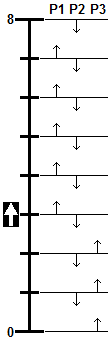
\includegraphics{P1_P2_P3_illustration.png}
	\caption{Grouping of Hall Calls to P1, P2 and P3}
	\label{p1p2p3}
\end{figure}

The behaviour of cars is governed precisely by the following three rules:
\begin{itemize}
	\item If a passenger in an elevator car has requested to get off at a particular floor, the car must not pass that floor without stopping.
	\item If a hall call has been allocated to a car, the car must not pass the floor of the call in the direction of the call without stopping.
	\item If there are passengers in a car, the car must not change direction.
\end{itemize}

\subsubsection{Control Logic}

Since the decision was made to use a discrete event-based simulation, it was necessary to consider how the movement of the cars, which is inherently continuous, could be represented meaningfully in a discrete manner.  While developing a dynamic programming approach to elevator scheduling, Nikovski and Brand [REF] present a discretised model of the state space of an elevator car in terms of its position in the shaft, which has been adapted for use in this simulator.  If one considers the two parameters of the continuous state space to be current speed and vertical position in the shaft then, given that the car will have some pre-determined maximum speed and rates of acceleration and deceleration, it can be seen that the car will follow certain fixed paths around this state space.  

Figure \ref{shaftstates} gives an example of a possible state space for an upward-travelling car, where the red dots represent the states, the green lines the transitions between states, and the blue lines the paths of deceleration from each state to its associated floor.  Each state can be thought of as a decision-point for its associated floor, at which the car decides whether to start slowing down in order to stop at the associated floor, or to carry on travelling upwards to the next decision point).  In this example, the floors are spaced evenly, but one can imagine how the states might look otherwise.  In any case, since each state lies on one of the blue deceleration paths, the parameters of a state can be determined from the floor with which it is associated, the movement speed associated with the state, and the specified rate of deceleration of the car.  A similar diagram could be drawn for a downward-moving car.

\begin{figure} [h]
	\centering
	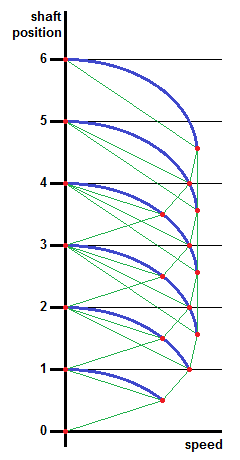
\includegraphics{shaft_state_space.png}
	\caption{The discretised state space of an upward-travelling elevator car}
	\label{shaftstates}
\end{figure}

As well as the floor, speed and direction, the state of the car contains two other parameters.  These are an action and a Boolean representing whether or not the doors are open.  While the latter is self-explanatory, the car action parameter requires some explanation.  The ten possible actions are defined in an enumeration called CarAction, and are described below:
\begin{description}
	\item[Leaving] The car state has this action when the car is accelerating away from having stopped at one floor and moving towards the decision point for the next floor.
	\item[Moving] This action is when the lift is passing a floor; it is moving, but it has not just left a floor, neither is it stopping at one.
	\item[Stopping] This action is when the lift has passed a decision point and decided to stop at the associated floor.
	\item[DoorsOpening] The car state has this action during the time that the car is opening its doors.
	\item[Unloading] This action is used for the time when passengers are getting out of the car.
	\item[Reversing] This action is used for the delay caused by a car configuring itself to move in the opposite direction.  The time of this action can be set to zero if changing the direction of a car incurs no delay, but previous literature assumes some delay will be caused.
	\item[Loading] Used during the time when passengers are boarding the car.
	\item[DoorsClosing] Used during the time when the car is closing its doors.
	\item[Idle] None of the above actions are currently taking place.
	\item[Stopped] This is something of a placeholder action, in that it does not represent any particular domain concept.  However, it does hold the logic to decide which of the above actions to enter next (as shown in Figure \ref{caractions}).
\end{description}

\begin{figure} [h]
\centering
	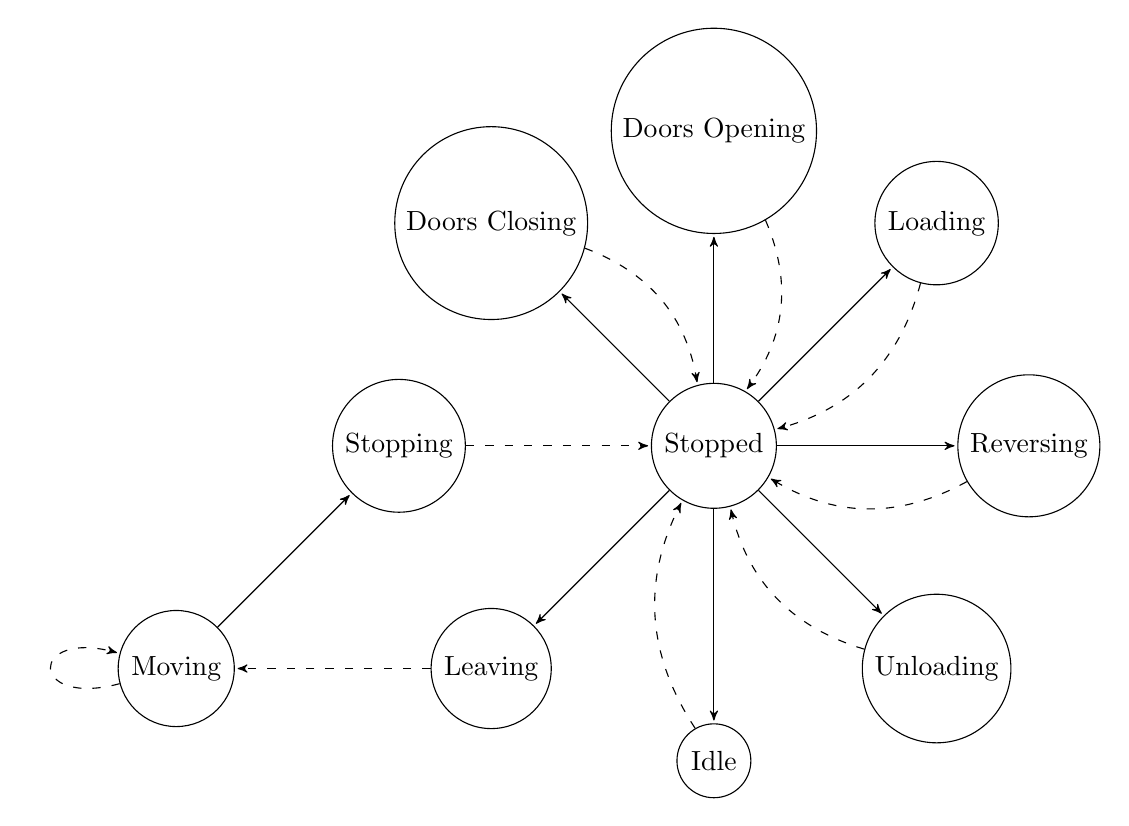
\begin{tikzpicture}[>=stealth',shorten >=1pt,auto,node distance=4cm]
		\node[state]	(stpd)						{Stopped};
  		\node[state] (drop)		[above of =stpd]		{Doors Opening};
  		\node[state] (load)		[above right of =stpd]	{Loading};
  		\node[state] (revs)		[right of =stpd]		{Reversing};
  		\node[state] (unld)		[below right of =stpd]	{Unloading};
  		\node[state] (idle)		[below of =stpd]		{Idle};
  		\node[state] (leav)		[below left of =stpd]	{Leaving};
  		\node[state] (movg)	[left of =leav]		{Moving};
  		\node[state] (stpg)		[left of =stpd]		{Stopping};
  		\node[state] (drcl)		[above left of =stpd]	{Doors Closing};
  		
  		\path[->]
  		(stpd)		edge	[]			node	{}	(drop)
  				edge	[]			node	{}	(load)
  				edge	[]			node	{}	(revs)
  				edge	[]			node	{}	(unld)
  				edge	[]			node	{}	(idle)
  				edge	[]			node	{}	(leav)
  				edge	[]			node	{}	(drcl)
		(movg)	edge	[]			node	{}	(stpg)
  		;
  		
  		\path[->, dash pattern = on 3pt off 4pt]
  		(drop)		edge	[bend left]		node	{}	(stpd)
  		(load)		edge	[bend left]		node	{}	(stpd)
  		(revs)		edge	[bend left]		node	{}	(stpd)
  		(unld)		edge	[bend left]		node	{}	(stpd)
  		(idle)		edge	[bend left]		node	{}	(stpd)
  		(leav)		edge	[]			node	{}	(movg)
  		(stpg)		edge	[]			node	{}	(stpd)
  		(drcl)		edge	[bend left]		node	{}	(stpd)
  		(movg)	edge	[loop left]		node	{}	(movg)
  		;
	\end{tikzpicture}
	\caption{A transition diagram of the car action element of a car state}
	\label{caractions}
\end{figure}

Figure \ref{caractions} demonstrates the relationship between the ten car action states.  In this diagram, solid transition edges denote immediate action changes, while dotted lines denote state changes that are made via the agenda.  For example, if the car is in the Stopped state, and determines that the next required action is to reverse, it will immediately change its state to Reversing.  Since there must then be a delay before the car can do anything else (specified by the user as, for example, 1 second), it will add an event on the agenda for 1 second later.  This agenda event will tell the car to go back into the Stopped state.  Then it might determine that the next required action is to load passengers, so it will immediately change into the Loading state.  It will then calculate the amount of time that loading will take (based on the number of passengers to load, and the user-specified loading time per passenger) and add an event onto the agenda for when the car should re-enter the Stopped state.  Putting future events onto the agenda allows the immediate control to return to the main control loop, which can (if appropriate) serve Passenger Hall Call events and/or events for other cars in the mean time.

\subsubsection{Movement Mathematics}

When the car is in one of the Leaving, Moving and Stopping action states, the car must work out the parameters of its next state.  If the current state is Leaving or Moving, then the next state will be a decision point for whether or not to stop at the next floor.  If the current state is Stopping, then the next state will be Stopped at the next floor.  In each case, we know all of the following information:

\begin{tabular}{l l}
	$U$ & The current speed (ms\textsuperscript{-1}) \\
	$F$ & The current floor \\
	$G$ & The next floor \\
	$S$ & The distance to the next floor (m) \\
	$A$ & The rate of acceleration of the car (ms\textsuperscript{-2}) \\
	$D$ & The rate of deceleration of the car (\textit{positive} ms\textsuperscript{-2}) \\
	$M$ & The maximum speed of the car (ms\textsuperscript{-1})
\end{tabular}

We are required to find the following parameters, which define our next state:

\begin{tabular}{l l}
	$V$ & The speed of the car when it reaches that state (ms\textsuperscript{-1}) \\
	$T$ & The time taken to reach the state (s)
\end{tabular}

In each case, we use the following basic equations of motion:

\begin{equation} \label{motioneq1} v=u+at\end{equation}
\begin{equation} \label{motioneq2} v^2=u^2+2as\end{equation}
\begin{equation} \label{motioneq3} s=ut+\frac{1}{2}at^2\end{equation}

In these equations, the variables are generically defined as follows:

\begin{tabular}{l l}
	$t$ & The duration of a time interval (s) \\
	$s$ & The distance travelled during the time interval (m) \\
	$u$ & The speed at the beginning of the time interval (ms\textsuperscript{-1}) \\
	$a$ & The rate of acceleration (ms\textsuperscript{-2}) \\
	$v$ & The speed at the end of the time interval (ms\textsuperscript{-1})
\end{tabular}

Once $V$ and $T$ have been found, the next car state will be placed on the agenda for $T$ seconds from now.

Here, I will demonstrate the maths for upward movement.  The maths for downward movement is analogous.

\paragraph{Moving state}

The Moving state applies when the car is moving, has reached a decision point, and has decided not to stop.  The parameters of the next decision point must be calculated, and there are two scenarios that must be considered.

The first, and simplest, scenario is where the car will accelerate until it reaches the decision point for the next floor, then decide whether or not to start slowing for the floor.  In this case, we simply need to find the point Q at which the acceleration curve from our current state crosses the deceleration curve for the next floor (Figure \ref{movingsimp}).

\begin{figure} [h]
	\centering
	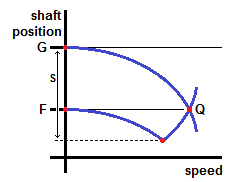
\includegraphics{moving_simp.png}
	\caption{Simple case while moving}
	\label{movingsimp}
\end{figure}

We first find the distance from here to point $Q$, which we will call $Q_D$.  By two applications of equation \ref{motioneq2} we find that:
\[Q_V^2=U^2+2AQ_D \text{ (for the acceleration curve)}\]
\[ \text{and } 0=Q_V^2-2D(S-Q_D) \text{ (for the deceleration curve).} \]

Note that $Q_V$ is the speed that we will have at point $Q$.  Combining these two equations we find that
\[ Q_D=\frac{2DS-U^2}{2(A+D)} \]

It is now trivial to find $V$ and $T$ as required, since
\[ V^2=Q_V^2=U^2+2AQ_D \text{ from equation \ref{motioneq2}} \]
\[ \text{and } T=Q_T=\frac{Q_V-U}{A} \text{ from equation \ref{motioneq1}. } \]

The second scenario is invoked when we find that $Q_V$ exceeds the maximum speed $M$ that our car can travel at.  In this case we will accelerate to some point $P$ on the acceleration curve (at which $P_V=M$), then move at a constant speed of $M$ until we reach the decision point $R$, the latest point at which we can decelerate to the next floor from speed $M$ (Figure \ref{movingcomp}).

\begin{figure} [h]
	\centering
	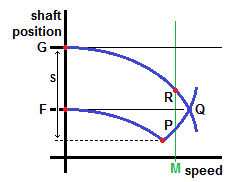
\includegraphics{moving_comp.png}
	\caption{Complex case while moving}
	\label{movingcomp}
\end{figure}

The parameters of the point $P$ on our acceleration curve are trivial to find:
\[ P_V=M \text{ by definition,} \]
\[ P_T=\frac{P_V-U}{A} \text{ from equation \ref{motioneq1}} \]
\[ \text{and } P_D=UP_T+\frac{1}{2}AP_T^2 \text{ from equation \ref{motioneq3}.} \]

Then, the distance from our initial point to point $R$, named $R_D$, can be found from the following equation
\[ 0=R_V^2-2D(S-R_D) \text{ from equation \ref{motioneq2},} \]
which rearranges to give
\[ R_D = S - \frac{R_V^2}{2D} \text{.} \]

Then, since the movement from $P$ to $R$ is constant at speed $M$ the required values $V$ and $T$ can be calculated as
\[ T = R_T = P_T+\frac{R_D-P_D}{M} \]
\[ \text{and } V = R_V = M \text{.} \]

Note that the above logic and equations also hold for the common case where the current speed of the car is already at the maximum speed.  In such a scenario, it is correctly calculated that $P_T=P_D=0$.

\paragraph{Leaving state}

The Leaving state applies when the car is stopped and about to start leaving.  The parameters of the first decision point that will be encountered by the car must be calculated.  The logic and equations for the Leaving state are the same as those for the Moving state, but if the car is in the Leaving state then $U=0$.  Figure \ref{leavingsimp} and Figure \ref{leavingcomp} demonstrate these scenarios graphically.

\begin{figure} [h]
	\centering
	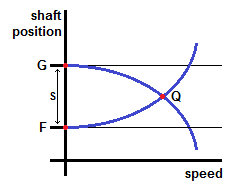
\includegraphics{leaving_simp.png}
	\caption{Simple case while leaving}
	\label{leavingsimp}
\end{figure}

\begin{figure} [h]
	\centering
	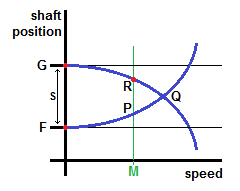
\includegraphics{leaving_comp.png}
	\caption{Complex case while leaving}
	\label{leavingcomp}
\end{figure}

\paragraph{Stopping state}

The Stopping state applies when the car is moving, has reached a decision point, and has decided to stop.  If the car is in the Stopping state, the maths is very simple.  The next state is reached by following the deceleration curve straight down to stopping at the floor.  Therefore,
\[ V=0 \text{ by definition of Stopping} \]
\[ \text{and } T=\frac{U}{D} \text{ from equation \ref{motioneq1}.} \]

\subsection{Allocator Component}

The Allocator component in the Core Elevator Simulator consists of an Interface class, named IAllocator, defining the methods that an Allocator implemented by the user must include.  In fact, the IAllocator interface is very simple and contains just one method which is called by the main control loop when a new PassengerGroup arrival is taken from the agenda:

\lstset{language=[Sharp]C, basicstyle=\ttfamily\tiny, breaklines=true, breakatwhitespace=true }
\begin{lstlisting}
interface IAllocator
{
	/// <summary>
	/// Allocates a given group of passengers to a specific car within
	/// the given building, based on the relevant allocation method
	/// </summary>
	/// <param name="group">The PassengerGroup to be allocated</param>
	/// <param name="building">The Building holding the domain model</param>
	void AllocateCall(PassengerGroup group, Building building);
}
\end{lstlisting}

There is also an enum class, AllocatorType, which defines the names of all of the allocators.  Then, there is a static method which takes a specific AllocatorType enum value and returns an instance of the relevant Allocator as implemented by the user.

In order to demonstrate the ease with which a new Allocator can be added, I will include an example of a very simple allocation algorithm, the ClosestCar algorithm, which simply allocates each call to whichever car is closest to the call at the time the call is made, ignoring the directions in which cars are moving.

Firstly, the user must create a new class, which implements IAllocator.  As described, the AllocateCall method must be implemented, as follows:

\begin{lstlisting}
class ClosestCarAllocator : IAllocator
{
	/// <summary>
	/// Allocates a given group of passengers to a specific car within
	/// the given building, based on the ClosestCar allocation method
	/// </summary>
	/// <param name="group">The PassengerGroup to be allocated</param>
	/// <param name="building">The Building holding the domain model</param>
	public void AllocateCall(PassengerGroup group, Building building)
	{
		// compile list of all cars
		List<ICar> cars = new List<ICar>();
		building.Shafts.ForEach(s => s.Cars.ForEach(c => cars.Add(c)));
		// get closest car
		var car = cars.OrderBy(c => Math.Abs(c.State.Floor - group.Origin)).First();
		// allocate call
		car.allocateHallCall(new HallCall(group));
	
		// update the PassengerGroup data with the time at which
		// the hall call was made
		group.changeState(PassengerState.Waiting, Simulation.agenda.getCurrentSimTime());
	}
}
\end{lstlisting}

Secondly, the name of the Allocator must be added to the AllocatorType enum:

\begin{lstlisting}
enum AllocatorType
{
	Manual,
	Random,
	ClosestCar
}
\end{lstlisting}

Finally, the new Allocator must be added to the mapping method:

\begin{lstlisting}
public static IAllocator getAllocator(AllocatorType allocator)
{
	switch (allocator)
	{
		case AllocatorType.Manual:
			return new ManualAllocator.ManualAllocator();
		case AllocatorType.Random:
			return new RandomAllocator.RandomAllocator();
		case AllocatorType.ClosestCar:
			return new ClosestCarAllocator.ClosestCarAllocator();
	}
	
	return null;
}
\end{lstlisting}

Once the user has performed these three steps, the simulator can be recompiled and the new Allocator can be used.

\subsection{Passenger Distribution Generator}

The purpose of the Passenger Distribution generator is to load an XML `specification' file, which contains the parameters of the Poisson distributions for the various floors.  Based on this, it outputs a second XML file containing a list of specific passenger groups, with their arrival times, sizes, origins and destinations.  The arrival times of these passenger groups should follow the relevant Poisson distributions as taken from the specification file.  An example specification file is shown below.

\lstset{language=XML}
\begin{lstlisting}
<ArrivalFloors>
	<ArrivalFloor Floor="0">
		<DestinationFloor Floor="1" ArrivalsPerMinuteMean="5.0" GroupSizeMean="2" />
		<DestinationFloor Floor="2" ArrivalsPerMinuteMean="3.0" GroupSizeMean="2" />
	</ArrivalFloor>
	<ArrivalFloor Floor="1">
		<DestinationFloor Floor="0" ArrivalsPerMinuteMean="0.5" GroupSizeMean="1" />
		<DestinationFloor Floor="2" ArrivalsPerMinuteMean="1.0" GroupSizeMean="1" />
	</ArrivalFloor>
	<ArrivalFloor Floor="2">
		<DestinationFloor Floor="0" ArrivalsPerMinuteMean="0.3" GroupSizeMean="1" />
		<DestinationFloor Floor="1" ArrivalsPerMinuteMean="0.5" GroupSizeMean="1" />
	</ArrivalFloor>
</ArrivalFloors>
\end{lstlisting}

This example specification is for up-peak traffic between three floors.  The first <ArrivalFloor> element specifies the mean number of arrivals per minute at floor 0 as 5 groups going to floor 1, and 3 groups going to floor 2.  Similarly, the mean is 0.5 groups per minute going from floor 1 to 0, and 1 group per minute going from 1 to 2.  0.3 groups per minute go from floor 2 to 0, while 0.5 groups per minute go from 2 to 1.  You will also see that the sizes of groups boarding at floor 0 are generally larger, with an average of 2 people as opposed to an average of 1 person per group for other movements.

The passenger distribution generator was run with the above specification file, and configured to create a schedule for a period of 10 minutes, from 13:00:00 to 13:10:00.  An extract from the file is shown here, but the full schedule is available in the appendix.

\begin{lstlisting}
<PassengerGroups>
	<PassengerGroup ArrivalTime="03/03/2014 13:00:02" Size="1" Origin="0" Destination="2" />
	<PassengerGroup ArrivalTime="03/03/2014 13:00:11" Size="2" Origin="0" Destination="1" />
	<PassengerGroup ArrivalTime="03/03/2014 13:00:20" Size="1" Origin="1" Destination="2" />
	<PassengerGroup ArrivalTime="03/03/2014 13:00:28" Size="2" Origin="0" Destination="1" />
	<PassengerGroup ArrivalTime="03/03/2014 13:00:31" Size="2" Origin="0" Destination="1" />
	<PassengerGroup ArrivalTime="03/03/2014 13:00:34" Size="2" Origin="0" Destination="1" />
	<PassengerGroup ArrivalTime="03/03/2014 13:00:48" Size="2" Origin="1" Destination="2" />
	<PassengerGroup ArrivalTime="03/03/2014 13:00:50" Size="1" Origin="0" Destination="1" />
	<PassengerGroup ArrivalTime="03/03/2014 13:00:52" Size="3" Origin="0" Destination="2" />
	<PassengerGroup ArrivalTime="03/03/2014 13:00:59" Size="1" Origin="0" Destination="2" />
	<PassengerGroup ArrivalTime="03/03/2014 13:01:12" Size="1" Origin="2" Destination="1" />
	<PassengerGroup ArrivalTime="03/03/2014 13:01:15" Size="4" Origin="0" Destination="1" />
	<PassengerGroup ArrivalTime="03/03/2014 13:01:51" Size="2" Origin="0" Destination="1" />
	<PassengerGroup ArrivalTime="03/03/2014 13:01:52" Size="1" Origin="0" Destination="1" />
	<PassengerGroup ArrivalTime="03/03/2014 13:02:31" Size="3" Origin="0" Destination="2" />
	<PassengerGroup ArrivalTime="03/03/2014 13:02:54" Size="2" Origin="0" Destination="2" />
	.
	.
	.
</PassengerGroups>
\end{lstlisting}

The format of this file is fairly straightforward; each Passenger Group in the schedule is shown as a single element in the file, with attributes storing its time of arrival, size, origin and destination.  This file is loaded at the start of a simulation run and all of the Passenger Group arrivals are added to the agenda.

\subsubsection{Generating values with a Poisson distribution}

The schedule is generated by using Knuth's algorithm \textbf{[CITATION]} for Poisson distributions, which is described by the following pseudocode:

\begin{lstlisting}
function PoissonDistributedRandomNumber(mean):
	L := e ^ (mean * -1)
	k := 0
	p := 1

	do while p > L:
		k := k + 1
		u := random[0, 1] // u is a random real number in the interval [0, 1]
		p := p * u

	return k - 1
\end{lstlisting}

When generating the schedule, we progress through time in steps specified by the user (in this example we will use 1 second time slices).  At each time step, we calculate the mean number of passenger groups for each movement in that time step (for a 1 second step, we divide the mean per minute by 60), and then use Knuth's algorithm to determine, based on that mean, how many arrivals we will have for each movement.  Then, for each arrival that we generate, we run Knuth's algorithm based on the mean group size for that movement to determine the size of the group.  The user specifies a maximum group size; if the size of a group is not between 1 and the user-specified maximum, we generate another value using Knuth's algorithm.

\subsection{Simulation Configuration}
All parameters of a simulation run are specified in a single configuration file, so that this configuration can be easily stored and re-run at a later date if desired.  A sample configuration file is shown in the appendix, but it includes the following parameters:
\begin{itemize}
	\item \textbf{Allocator} -- the name of the allocator that is to be used
	\item \textbf{Passenger Distribution parameters}
	\begin{itemize}
		\item Whether to load an existing distribution file or create a new one based on a given specification file
		\item Specification file path (if generating a new distribution)
		\item Maximum Passenger Group size (if generating a new distribution)
		\item Start time of distribution (if generating a new distribution)
		\item End time of distribution (if generating a new distribution)
		\item Resolution; the size of time steps (if generating a new distribution)
		\item Distribution file path
	\end{itemize}
	\item A selection of named sets of \textbf{Car Attributes}
	\begin{itemize}
		\item Maximum capacity
		\item Maximum speed
		\item Acceleration
		\item Deceleration
		\item DoorsOpenTime -- time taken to open doors
		\item DoorsCloseTime -- time taken to close doors
		\item DirectionChangeTime -- time taken to reverse
		\item PassengerBoardTime
		\item PassengerAlightTime
	\end{itemize}
	\item The domain model \textbf{Building}, with its lowest and highest floors, and the distance between floors specified.
	\begin{itemize}
		\item A selection of \textbf{Shafts}, within which
		\begin{itemize}
			\item A selection of \textbf{Cars}, each of which is linked to a set of Car Attributes as defined above, and a CarType (always Single-decker in the Core Elevator Simulator) as well as the floor at which the car is to be initialised.
		\end{itemize}
	\end{itemize}
	\item The path to a \textbf{Log File} -- the user can specify `auto' here, in which case an automatic file name will be generated based on the current date and time.
\end{itemize}

\section{Validation}

\textit{All validation work was performed independently of Craig, as were the code corrections made in response.}

The architecture of the Core Elevator Simulator allows each component to be validated separately, with only minimal verification on the ways in which they interact.

\subsection{Domain Model Component}

The most significant component to validate is the Domain Model component.  In order to test it I designed a specific passenger arrival schedule, containing a total of 13 groups and 39 passengers arriving over the course of 2\textonehalf minutes, that would result in each workflow within the Car domain logic being tested.  The test modelled a building with just 3 floors, since this was enough to give confidence about the performance over a larger number without increasing the complexity of the hand-calculations.  Since the cars do not interact with each other in the Core Elevator Simulator, I built a dummy allocator that would assign all calls to car 0, meaning that all calls would be handled by the same car. \textbf{[These two points must be tested at least a little]}

Using Microsoft Excel to maintain a trace table, I worked through the way in which the car should behave as the different calls came in, performing all of the movement calculations and other mathematics by hand.  I calculated that the simulation run with my designed passenger arrival schedule would take 4 minutes and 14 seconds, and noted down the specific boarding and alighting times of each Passenger Group.  I also had a record of every state change that would take place in the car during the simulation run, which is shown in the appendix.

The test run included two scenarios where the car could not serve the calls due to lack of capacity, and it handled this correctly.  It also included cases where hall calls came in as the doors were closing.  The expected behaviour was for the car to reopen the doors and serve the hall calls before leaving.

There were times when the car would set off from floor 2, heading to floor 0 and then a hall call would come in at floor 1 just after it had left.  In this case, the expected behaviour was for the car to make an unexpected stop at floor 1, as long as the call came in before the car had passed the final decision point for floor 1.

Initially, when I ran the simulator for the first time on the specific passenger arrival schedule I was encouraged to see that for the first 45 seconds, the logs showed that the car was behaving exactly as I had predicted that it should in the trace table.  Unfortunately, after that the timings became about half a second out, which was the indicator of some flawed logic either in the simulator itself or in my hand-calculated trace table.  Having seen that the discrepancy came on the first occasion that the car was directed to pass a floor without stopping, I placed a breakpoint in that logic to find out if there was any problem.

In fact, there was a problem.  I had erroneously implemented the formula for finding PD as follows
\[ P_D = U + \frac{1}{2}AP_T^2 \text{,} \]
when, in fact, the correct formula is slightly different, as follows
\[ P_D = UP_T + \frac{1}{2}AP_T^2 \text{.} \]

After I had corrected this implementation, I tried the simulation run again and this time found that everything was behaving as expected.  All of the car state changes happened at the right time (within the 10-millisecond accuracy to which I had done my hand calculations), and all of the passenger boarding and arrival times were as expected too.  I am now confident that the Domain Model component of the Core Elevator Simulator behaves correctly.

\subsection{Allocator Component}

Since the Allocator component will be re-implemented for each allocation algorithm that is run on the simulator, it doesn't really make sense to completely validate it at this stage.  However, in order to test the general interactions between the Allocator and the Domain Model component I have used the basic ClosestCar allocator as described above.  I then used a Manual allocator, which asks the user to allocate calls to cars, to make the decisions in my head (in the way that I believe the ClosestCar allocator should allocate them) and ensure that the behaviour of the simulator when using the ClosestCar allocator matches the behaviour when I make the decisions myself.

After running the simulation in both scenarios (with the same passenger arrival schedule as used in the domain model component tests), I found that the logs were identical.  Therefore, I am confident that the allocator component is behaving as it should.  It would not be useful to print the entire log here, but I will print the evaluation results which can be used for later verification if necessary:

\begin{lstlisting}
Average waiting time:                4.92269230769231
Average squared waiting time:        126.226432384615
Average time to destination:         22.3131538461538
Average squared time to destination: 782.275027153846
Longest waiting time:                38.249
Longest time to destination:         66.667
\end{lstlisting}

When the simulator is used with new allocation algorithms, care should be taken to ensure that the new Allocators have been implemented correctly, and tests should be performed to validate the implementations.

\chapter{TCOS Elevator Simulator}
\label{teschapter}

\section{Introduction}

This chapter describes the portion of the project during which I extended the Core Elevator Simulator to work for the Two Cars in One Shaft (TCOS) case.

\section{Additional Requirements}

\subsection{Specification of Requirements}

The following is a list of additional requirements that had to be met by the TCOS Elevator Simulator.  All of the requirements for the Core Elevator Simulator still applied, but will not be listed again here.  The only exception was that the requirement to be able to simulate systems \textit{without} Destination Control no longer applied, since TCOS systems always use Destination Control.

\subsubsection{Functional Requirements}

	\begin{enumerate}
		\item To be able to simulate the use, and evaluate the performance, of algorithms designed for the allocation of calls to cars in TCOS elevator systems.  The evaluation objectives must include those specified in the requirements for the Core Elevator Simulator.
		\item It should be possible to use, in one simulation, traditional elevator shafts (with exactly one car) and TCOS elevator shafts.
		\item In TCOS shafts, there should be a `garage' floor below the ground floor, in which the lower car can park, leaving the upper car with access to all passenger floors.
		\item Cars should have an optional `parking' behaviour so that when they become Idle they move to wait at a specific floor rather than just waiting in their current location.
		\item In TCOS shafts, the lower car should not accept call allocations which include the highest floor.  There is no restriction on which calls the upper car can accept.
	\end{enumerate}

\subsubsection{Non-Functional Requirements}

	\begin{enumerate}
	\setcounter{enumi}{5}
		\item The TCOS extension should avoid changes to the existing code that are so significant as to prevent re-integration with the Core Elevator Simulator line.  This will allow the TCOS simulator to be combined with other extensions made in parallel, making a single general purpose simulator.
		\item The TCOS extension should be built in such a way that it can be further extended to handle Many Cars in One Shaft (MCOS) cases (i.e. cases where a single shaft might contain 3 or more cars).
	\end{enumerate}

\subsection{Justification of Requirements}

The above requirements are justified as follows.

Requirement 1 specifies that the same evaluation objectives should be used in the TCOS Elevator Simulator as in the Core Elevator Simulator.  The reason for this is that it allows direct comparisons to be made between the performance of elevator groups containing TCOS shafts and those only containing traditional shafts.  With these comparisons available, inferences could be made about the scenarios in which TCOS systems can provide better performance than traditional systems.

In some scenarios, a building operator might choose to upgrade some subset of their elevator shafts to TCOS, while leaving the remaining shafts operating in the traditional manner.  Requirement 2 allows different such scenarios to be evaluated.

The garage floor in requirement 3 allows the lower car in a TCOS shaft to park out of the way, so that the upper car can visit all floors.  The parking functionality in requirement 4 allows the Allocator to make use of this floor, as well as having the upper car automatically park at the top floor so as to maximise the floors available to the lower car.

Requirement 5 stops the deadlock situation whereby a call for the top floor is allocated to the lower car, which can never reach the call due to the presence of the upper car.

Requirements 6 and 7 are included to ensure that the TCOS Elevator Simulator can be put to best use by me and others following the end of this project.

\section{Domain Assumptions}

There are a number of assumptions made about the TCOS case in addition those made for the Core Elevator Simulator.
	\begin{enumerate}
		\item The separation of cars within a shaft is controlled by ensuring that no two cars may occupy the same floor at the same time.
		\item When a car is moving from one floor ($a$) to the next ($b$), it is considered to occupy both floors at the same time.  Therefore the other car may not start moving towards floor $a$ until the car has reached floor $b$.
		\item No further separation is enforced between cars except as specified and implied by the assumptions above.
		\item No car will stop between floors.
	\end{enumerate}

\section{High Level Design Decisions}

The TCOS case introduced some complications to the constraints, which mean that decisions had to be made about the control logic in the Domain Model component.  Various strategies were considered in order to avoid deadlock or collision between cars.

\subsection{Option 1: Dynamic `Zoning' Approach}

This approach works by considering each car within a shaft to have an exclusive zone of floors transiently defined as the minimal set of consecutive floors containing (a) the current floor of the car, (b) the car's park floor, and (c) the locations of all calls currently assigned to the car.  When the Allocator attempts to assign a call to a car, the car must either accept or reject the call based on the following rules:
	\begin{enumerate}
		\item If both the origin and destination of the call are within the car's current zone, the call will be accepted.
		\item Otherwise, if both the origin and destination lie within the range of floors that the car's current zone can be extended into without overlapping with the zone of another car in the same shaft, the call will be accepted and the car's current zone will be extended accordingly.
		\item Otherwise, the call will be rejected and the Allocator will have to allocate the call to another car.
	\end{enumerate}

In this case, the park floors should be fixed as the highest floor (for the upper car) and the garage floor (for the lower car).

This approach very effectively separates the cars and does so without ultimately limiting the range of floors that any car can serve (for example, with appropriate Allocator behaviour, the upper car could conceivably serve a call at the ground floor, if the lower car is parked at the garage floor).  However, it is inefficient in that it could restrict the allocation of calls that might actually be feasible.  For example, if the upper car is at floor 8, and the lower car is travelling down from floor 4 to floor 1, it might be reasonable to allocate a call at floor 3 to the upper car.  This approach would not allow the allocation.

\subsection{Option 2: Conflict Resolution Approach}

This more complicated approach allows any call to be allocated to any car at any time, and then relies on the control logic to resolve conflicts between cars.  In general, there are two types of conflict: one where the cars are travelling in the same direction but the car in front is delaying the car behind and the other where the cars are both travelling towards each other.  The former of these is simple to resolve from a conceptual perspective – the one behind must wait for the other to move out of the way before proceeding.  The latter presents some issue as one car (a `slave') must reverse for some distance to allow the other one (the `master') to serve its calls.  Some method of determining which car would be given priority would be required in order to use this approach.

While this approach has the potential to solve the efficiency problem of option 1, it also has some problems of its own.  For example, the master-slave behaviour would result in some conflict with the passenger expectation constraints (i.e. that a car must not change direction if it currently has passengers on board).  Additionally, it means that some non-trivial logic which is conceptually part of the allocation process is fixed within the Domain Model component.

\subsection{Option 3: Overlapping Dynamic Zoning Approach}

The third option is similar to option 1, but it allows the zones of the two cars to overlap as long as the zone of the upper car does not contain the current floor of the lower car and vice-versa.  In this case, the set of floors that are in the zones of both cars is known as the overlap zone.  Only one of the cars may enter the overlap zone at a time, and this permission is granted to whichever one gets there first.  For example, if the overlap zone is floors 4, 5 and 6, and the lower car attempts to visit floor 4 while the upper car is still at floor 8, the lower car will continue to floor 4 and subsequently floors 5 and 6.  In the meantime, the upper car will be held at floor 7.  When the lower car leaves floor 6 to return to floor 5 the overlap zone will now only contain floors 4 and 5, so the upper car will be allowed to proceed to floor 6, and so on.

The following rules would be used to decide whether or not to accept a hall call:
\begin{enumerate}
	\item If both the origin and destination of the call are within the car's current zone, the call will be accepted.
	\item Otherwise, if the car's current zone contains a floor already occupied by the other car in the shaft, and both the origin and destination of the call are within the other car's zone without being the last floor in its zone, the call will be accepted and the car's current zone will be extended accordingly.
	\item Otherwise, if both the origin and destination lie within the range of floors that the car's current zone can be extended into without including the current floor of the other car in the same shaft, the call will be accepted and the car's current zone will be extended accordingly.
	\item Otherwise, the call will be rejected and the Allocator will have to allocate the call to another car.
\end{enumerate}

Note that if one car has already entered the overlap zone, the second rule allows the waiting car's zone to expand further past the other car.  This does not cause any problem, so long as the other car's zone always protrudes at least one floor further so as to avoid deadlock occurring later on.

As with option 1, the park floors for the upper and lower cars should be the highest floor and the garage floor respectively.

Option 3 is more efficient than option 1 in that it allows some feasible call allocations that option 1 does not allow.  However, it manages to extend the possibilities without contravening the passenger expectation constraints or the conceptual logic architecture of the simulator.

\subsection{Option 4: Extended Overlapping Dynamic Zoning Approach}

The fourth option considers that a car's zone is the minimal set of floors that contains (a) the current floor of the car, (b) the car's park floor, and (c) all floors that the car will visit before its next reversal.  This is different from the zones defined in options 3 and 4 as it only includes the calls in P1 and, if it is beyond the furthest location of all P1 calls, the first call in P2.

This option extends option 3 to allow one car's zone to `absorb' the current floor of the other car, provided that the other car's zone does not already include this car's current floor (i.e. this car is not inside the overlap zone).  The result of this absorption is that the other car is now inside the overlap zone, and thus this car must wait for the other car to leave before it can enter.

The changes to the zone definition mean that if a car is travelling towards its park floor, none of the floors behind it are included in its zone, meaning that the other car can follow it if it wants to without ending up in the situation where both cars are in the overlap zone.  However, in order to avoid a deadlock situation, if the car is travelling towards its park floor it must continue to do so until it has left the zone of the other car before reversing, so as to allow the other car to attend its calls.

In this option, the rules for accepting and rejecting calls are as follows:
	\begin{enumerate}
		\item If the call is a P3 call, the call will be accepted.
		\item Otherwise, if both the origin and destination of the call are within the car's current zone, the call will be accepted.
		\item Otherwise, if the car's current floor is not inside the overlap zone, and both the origin and destination of the call are within the other car's zone without being the last floor in its zone, the call will be accepted and the car's current zone will be extended accordingly.
		\item Otherwise, if the car's current floor is inside the overlap zone, and both the origin and destination lie within the range of floors that the car's current zone can be extended into without including the current floor of the other car in the same shaft, the call will be accepted and the car's current zone will be extended accordingly.
		\item Otherwise, the call will be rejected and the Allocator will have to allocate the call to another car.
	\end{enumerate}

Note that the lower car can never accept a call that requires it to visit the highest floor, and the upper car can never accept a call that requires it to visit the garage floor.  This rule is implicitly satisfied by the rules given above (a car cannot accept a call where either the origin or destination floor is the last floor in the other car's zone).

Again, the park floors for the upper and lower cars should be the highest floor and the garage floor respectively.

This option further builds on the benefits of options 1 and 3, without contravening either the passenger expectation constraints or the conceptual logic architecture of the simulator.  For this reason, I chose to use option 4 in the TCOS Elevator Simulator.

\section{Detailed Description of Changes Made}

In this section I will describe the changes that were necessary in order to extend the Core Elevator Simulator for the TCOS case.  The majority of the changes were to the Domain Model component, though minor changes were also necessary in the Allocator and Simulation Configuration components.

\subsection{Domain Model Component}

There was a large amount of logic that needed to be added to the Domain Model in the TCOS Elevator Simulator.  In order to maintain the generality of the simulator (so that it could still be used for simulations including traditional elevator shafts as well as TCOS shafts) a new TCOSCar class was added, and the traditional Car class was left largely unchanged.  The Core Elevator Simulator had been designed such that the traditional Car class implemented an interface, ICar, and all interactions with the Car were via the ICar interface.  This meant that the TCOSCar class simply needed to interface the ICar interface in order to be compatible with the rest of the program.

Since the Extended Overlapping Zoning Approach (option 4, discussed above) requires that a TCOS car can reject call allocations, it was necessary to modify the ICar interface slightly so that the allocateHallCall method, called by Allocators to allocate a call to a car, returned a Boolean value indicating the success (true) or failure (false) of the allocation.  The traditional Car class had to be modified accordingly, simply returning true (for success) in all cases.

Aside from the minor `housekeeping' changes described above, the following three methods were added in the TCOS implementation, corresponding to certain aspects of logic in option 4:
	\begin{description}
		\item[CanAcceptHallCall] Based on the rules described in option 4, this method works out whether or not a call can be accepted at the current time, based on the circumstances of both cars in the shaft and the calls currently allocated to them.
		\item[CanMoveToNextFloor] This method works out whether or not the car is permitted to move forward to the next floor.  This is necessary because a car cannot enter the overlap zone while the other car is within it.
		\item[MustContinueInCurrentDirection] This method works out whether or not the car must continue forward in order to allow the other car to visit its calls, even if this car needs to reverse before it can serve its own calls.  As described in option 4, if the car is in the overlap zone and travelling back towards its park floor it must continue forward until it has left the overlap zone, so as to avoid causing a deadlock situation.
	\end{description}
	
All of these three methods require knowledge of the current zones applicable to the two cars in the shaft.  Therefore, a CurrentZone property was added in the TCOSCar class, which calculates and returns a list of all floors in the current zone according the definition described in option 4.  Additionally, a CurrentFloorsOccupied property was added in the TCOSCar class, which returns a list of up to 2 floors that the car is currently occupying.  If a car is stopped at floor 4, this list only contains the value 4, while if it is moving from floor 4 to floor 5, the list contains both 4 and 5 until it arrives at floor 5 when it will contain just 5.

A new action was added to the CarAction options, named `Waiting', which a TCOS car uses when it is stationary waiting for the other car to perform tasks before it can move.  When one car in the shaft moves, it notifies the other car so that the other car can, if appropriate, re-assess the situation and decide whether or not to continue waiting.  The waiting car will begin moving again once the other car has started moving back towards its park floor.

It was also necessary to change the behaviour of the cars so that, instead of simply stopping in situ and changing its action to Idle when there are no calls to serve, the car would move to its designated park floor at this stage before entering changing to a new action, named `Parked'.

\subsection{Allocator Component}

The only change necessary in the Allocator component related to the fact that a car can now reject hall call allocations, with the allocation method returning true or false to indicate whether or not the allocation was accepted.  Therefore, Allocators must be aware of the potential for an allocation to fail and, if appropriate, implement code to handle an allocation failure and attempt allocation to another car.

\subsection{Simulation Configuration}

The first change necessary in the Simulation Configuration component was to allow simulation configuration files to specify the park floor of each car.  This was implemented by adding a ‘parkFloor’ attribute to the `Car' tag in the XML config files, the value of which is passed to the corresponding car at the start of the simulation.

The second change was to add `TCOS' as an option for the car type, so that the user could select to use TCOS cars in the simulation.

\section{Validation}

\subsection{Domain Model Component}
As with the Core Elevator Simulator, the most significant validation required in the TCOS Elevator Simulator is in the Domain Model component.  Again, since each car only interacts with the other car in its shaft, it was appropriate to focus the testing on the behaviour of cars within a single shaft.  This time, I used a building consisting of 10 floors, numbered 0 to 9, as well as a garage floor below floor 0 (numbered -1) which could not be used by passengers.  The passenger arrival schedule contained 9 passenger groups, totalling 39 people, arriving over the course of 2\textonehalf minutes.  I built an allocator named TwoZonesAllocator which would allocate each hall call to either the upper or lower car depending on the origin and destination floors of the passenger group involved (if the average of the origin and destination was greater than or equal to 4.5 the allocator would first attempt to allocate it to the upper car, otherwise it would first attempt to allocate it to the lower car).  If the first allocation attempt failed, it would allocate it to the other car instead.

Again, I used Microsoft Excel to maintain a trace table of the behaviour of both cars in the shaft, performing all calculations by hand.  I calculated that the full simulation run would take a total of 4 minutes and 54 seconds, and kept a record of the boarding and alighting times of each passenger group.  The full trace table, including every state change that took place, is shown in the appendix.

The passenger arrival schedule was designed to invoke all of the code path scenarios available, specifically testing the following cases:
	\begin{itemize}
		\item A car stops to pick up passengers that cannot be accommodated due to lack of available space.  In this scenario the car was to revisit and attempt to pick up the passengers later on, and it was important that the zoning approach could handle this change of circumstances appropriately.
		\item A car is closing its doors when it receives a new call to be served from this floor in this direction.  The car was to reopen its doors and allow the new passengers on.
		\item A car receives a call requiring it to stop at the next floor, while it is currently moving towards that floor.  Provided there is still time to stop, the car is to make an unexpected stop to pick up the passengers.
		\item A car wishes to enter the overlap zone when the other car already occupies the zone.  The car must wait for the other car to turn back before it can continue.
		\item A car has finished serving all calls in P1 and needs to reverse in order to serve P2 calls.  However, the other car has entered the overlap zone and needs to come to the floor that this car currently occupies.  This car must first continue away from its calls so that the other car can serve its calls, so as to avoid a deadlock scenario.
		\item A car has finished serving all calls in P1, P2 and P3.  It must return to its park floor and wait for further calls to be allocated.
		\item A car is inside the overlap zone when the allocator attempts to allocate a P1 call that would require the car to visit the floor at which the other car is currently waiting.  Since this would result in a deadlock scenario, the car must reject the call.
	\end{itemize}

When I first ran the TCOS Elevator Simulator configured as described above, the two cars in the shaft entered a deadlock scenario.  This meant that either there was a problem with the logic decided upon in option 4 (extended overlapping dynamic zoning) or that it had been incorrectly implemented in the code.  I placed a breakpoint in the code to be activated just before the deadlock scenario occurred so that I could examine the implementation and determine the cause of the problem.  It turned out that the implementation of the logic in the MustContinueInCurrentDirection method was flawed in that it only considered the floor of the other car's state, even if the other car had been authorised to proceed to the next floor and was moving towards it.  I changed the code to use the CurrentFloorsOccupied property of TCOSCar which includes the floor towards which a car has started moving.

After I had corrected this aspect of the code, I ran the simulation again and found that everything behaved as expected.  The car state changes happened at the right times (within the 10-millisecond accuracy to which I had performed my calculations), and all passenger boarding and arrival times were as expected, as well as the success and failure of call allocations.  I am now confident that my changes to the Domain Model in the TCOS Elevator Simulator are valid.  \ref{tcosvalidationgraph} is an Excel-generated graph which shows the movement of the upper (pink) and lower (blue) cars with time, demonstrating the minimum distance maintained between the two cars.

\begin{figure} [h]
	\centering
	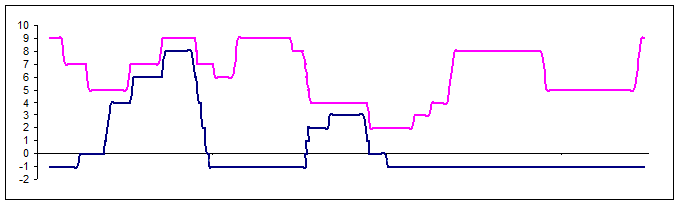
\includegraphics{tcos_validation_movement_graph.png}
	\caption{The movement of the two cars during the validating simulation run}
	\label{tcosvalidationgraph}
\end{figure}

\subsection{Allocator Component}
The only change to the Allocator component was for Allocators to handle call allocation failures from Cars.  This was implicitly tested during the Domain Model tests described above and performed correctly.  However, it is still necessary that each new Allocator that is implemented should be properly validated as discussed in the Core Elevator Simulator part.

\part{Algorithms for TCOS Elevator Systems}

\chapter{Discussion of Allocation Algorithms}

In this chapter, I will discuss a number of allocation algorithms that I have developed or adapted for use in the TCOS case.  In Chapters \ref{algsimchapter} and \ref{algtestchapter} I will describe the process of evaluating each of these algorithms on the TCOS Elevator Simulator, and discuss their performances.

\section{Estimated Time of Arrival (ETA)}

The Estimated Time of Arrival (ETA) algorithm is an existing algorithm for traditional elevator systems which has been widely studied in the literature \citep{Rong2003, Nikovski2003} and performed well in simulations \citep{Rong2003}.  The algorithm happens to work in such a way that its concepts can be adapted for use in the TCOS case.  After briefly describing ETA in its original form, I will discuss three ways in which I have adapted it for TCOS systems.

ETA is an immediate allocation algorithm that aims to minimise the average waiting time of all passengers in the system.  Every time a new hall call is made, it considers allocating the call to each one of the cars in the system and estimates the cost each of the possible allocations.  It then allocates the call to the car which results in the lowest estimated cost.  The cost estimation function of allocating the call to a given car is made up of two parts: the estimated time taken for the car to reach the new call (Estimated Waiting Time), and the total additional waiting time caused to the other passengers currently waiting for the car (System Degradation Factor) \citep{Rong2003}.  The Estimated Waiting Time and System Degradation Factor are summed together to provide the total estimated cost.

A simple modification to ETA allows allocation costs to be estimated based on squared waiting times, thus preferring a narrower spread of results over one where some individuals benefit highly and others are severely disadvantaged.

\citet{Rong2003} present a reallocation variant of ETA, which allows calls to be retrospectively reassigned after the initial assignment, but since this is not compatible with Destination Control systems I will not describe it here.  They also describe methods of predicting passenger destinations in systems without Destination Control, but since Destination Control gives us full knowledge of the intentions of passengers as soon as they have made hall calls there is no need for us to consider these methods.

ETA
P		SP		S		/
15		16		16		17
731		830		926		1077
68		71		69		71
6967	7373	6925	7376
311		291		280		299
429		372		357		367

ETD
P		SP		S		/
34		33		?		?
2198	2050			
68		69				
6303	6115			
249		221				
274		259				

\subsection{Na\"{i}ve ETA}

The simplest method of adapting ETA for TCOS systems is simply to apply the basic cost estimation function to each car in the system ignoring the interactions between two cars in the same shaft.  The method of calculating the approximate cost is as follows:

Assume the following given time parameters (all in seconds):

\begin{tabularx}{\linewidth}{l X}
	$Start$		& The time taken for a car to start moving from loading (including closing doors, additional time required for acceleration, etc.) \\
	$Stop$		& The time taken for a car to stop moving and start loading (including opening doors, additional time required for deceleration, etc.) \\
	$Travel$	& The time taken for a car to travel between floors once moving \\
	$Reverse$	& The additional time taken for a car to reconfigure its direction when stopped \\
	$Unload$	& The time taken for a single passenger to alight the car \\
	$Load$		& The time taken for a single passenger to board the car
\end{tabularx}

Using these time parameters, and the full knowledge of all passengers currently waiting for or travelling inside the car, predict, for each passenger group, the amount of time that they will have to wait before the car arrives to pick them up.  Then, consider allocating the new hall call to the car and the effect that this will have on the waiting times of the other passengers.  This effect is the System Degradation Factor (SDF) and can be stated as follows:
\[ SDF(c, h) = \sum\limits_{g \in G(c)} (EWT(g, c, G(c) \cup \left\{ h \right\}) - EWT(g, c, G(c)))\]
where $c$ is the car, $h$ is the new hall call to be allocated, $G(c)$ is the set of groups already allocated to car $c$ and $EWT(g,c,G(c))$ is the estimated time taken for car $c$ to reach call $g$ given the calls in $G(c)$ (estimated waiting time for $g$).

The total estimated cost of allocating call $h$ to car $c$ is as follows:
\[ Cost(c, h) = SDF(c, h) + EWT(h, c, G(c) \cup \left\{ h \right\}) \]

Estimated waiting times can be calculated en masse by doing a rough simulation of the behaviour of the elevator using the six time parameters above and noting the boarding times of each group.  It would be possible to perform this simulation more exactly by using the simulation methods employed by my own TCOS Elevator Simulator but this is computationally expensive and in real world applications allocation decisions must be quickly computable both to make the process more efficient from a customer perspective and to avoid the state of the system changing significantly during the course of the computation.  I consider that the small loss of accuracy from using an approximate method is unlikely to significantly affect the performance of the allocation algorithm, and the consequences of an occasional sub-optimal allocation are of less concern than the alternative risks.

\subsection{Conflict-sensitive ETA}

\subsection{Capacity-sensitive ETA}

\section{dddd}

\chapter{Simulation of Allocation Algorithms}
\label{algsimchapter}

\chapter{Evaluation of Allocation Algorithms}
\label{algtestchapter}

\bibliography{Resources}

\appendix
\part{Appendices}

\chapter{Materials referred to in Chapter \ref{ceschapter}}

\section{XML Materials}

\subsection{Sample Passenger Arrival Schedule file}

\lstset{language=XML}
\begin{lstlisting}
<PassengerGroups>
	<PassengerGroup ArrivalTime="03/03/2014 13:00:02" Size="1" Origin="0" Destination="2" />
	<PassengerGroup ArrivalTime="03/03/2014 13:00:11" Size="2" Origin="0" Destination="1" />
	<PassengerGroup ArrivalTime="03/03/2014 13:00:20" Size="1" Origin="1" Destination="2" />
	<PassengerGroup ArrivalTime="03/03/2014 13:00:28" Size="2" Origin="0" Destination="1" />
	<PassengerGroup ArrivalTime="03/03/2014 13:00:31" Size="2" Origin="0" Destination="1" />
	<PassengerGroup ArrivalTime="03/03/2014 13:00:34" Size="2" Origin="0" Destination="1" />
	<PassengerGroup ArrivalTime="03/03/2014 13:00:48" Size="2" Origin="1" Destination="2" />
	<PassengerGroup ArrivalTime="03/03/2014 13:00:50" Size="1" Origin="0" Destination="1" />
	<PassengerGroup ArrivalTime="03/03/2014 13:00:52" Size="3" Origin="0" Destination="2" />
	<PassengerGroup ArrivalTime="03/03/2014 13:00:59" Size="1" Origin="0" Destination="2" />
	<PassengerGroup ArrivalTime="03/03/2014 13:01:12" Size="1" Origin="2" Destination="1" />
	<PassengerGroup ArrivalTime="03/03/2014 13:01:15" Size="4" Origin="0" Destination="1" />
	<PassengerGroup ArrivalTime="03/03/2014 13:01:51" Size="2" Origin="0" Destination="1" />
	<PassengerGroup ArrivalTime="03/03/2014 13:01:52" Size="1" Origin="0" Destination="1" />
	<PassengerGroup ArrivalTime="03/03/2014 13:02:31" Size="3" Origin="0" Destination="2" />
	<PassengerGroup ArrivalTime="03/03/2014 13:02:54" Size="2" Origin="0" Destination="2" />
	<PassengerGroup ArrivalTime="03/03/2014 13:03:05" Size="1" Origin="0" Destination="1" />
	<PassengerGroup ArrivalTime="03/03/2014 13:03:12" Size="2" Origin="0" Destination="1" />
	<PassengerGroup ArrivalTime="03/03/2014 13:03:16" Size="3" Origin="0" Destination="1" />
	<PassengerGroup ArrivalTime="03/03/2014 13:03:19" Size="2" Origin="0" Destination="1" />
	<PassengerGroup ArrivalTime="03/03/2014 13:03:27" Size="1" Origin="1" Destination="2" />
	<PassengerGroup ArrivalTime="03/03/2014 13:03:30" Size="2" Origin="1" Destination="2" />
	<PassengerGroup ArrivalTime="03/03/2014 13:03:32" Size="2" Origin="1" Destination="2" />
	<PassengerGroup ArrivalTime="03/03/2014 13:03:36" Size="1" Origin="0" Destination="2" />
	<PassengerGroup ArrivalTime="03/03/2014 13:03:37" Size="2" Origin="0" Destination="2" />
	<PassengerGroup ArrivalTime="03/03/2014 13:03:43" Size="1" Origin="0" Destination="2" />
	<PassengerGroup ArrivalTime="03/03/2014 13:03:48" Size="2" Origin="1" Destination="0" />
	<PassengerGroup ArrivalTime="03/03/2014 13:03:52" Size="1" Origin="0" Destination="1" />
	<PassengerGroup ArrivalTime="03/03/2014 13:03:58" Size="3" Origin="0" Destination="1" />
	<PassengerGroup ArrivalTime="03/03/2014 13:04:02" Size="1" Origin="1" Destination="2" />
	<PassengerGroup ArrivalTime="03/03/2014 13:04:11" Size="1" Origin="0" Destination="1" />
	<PassengerGroup ArrivalTime="03/03/2014 13:04:38" Size="1" Origin="2" Destination="1" />
	<PassengerGroup ArrivalTime="03/03/2014 13:04:42" Size="4" Origin="0" Destination="1" />
	<PassengerGroup ArrivalTime="03/03/2014 13:04:45" Size="1" Origin="0" Destination="1" />
	<PassengerGroup ArrivalTime="03/03/2014 13:05:01" Size="1" Origin="1" Destination="2" />
	<PassengerGroup ArrivalTime="03/03/2014 13:05:06" Size="1" Origin="0" Destination="2" />
	<PassengerGroup ArrivalTime="03/03/2014 13:05:12" Size="1" Origin="0" Destination="1" />
	<PassengerGroup ArrivalTime="03/03/2014 13:05:12" Size="1" Origin="1" Destination="2" />
	<PassengerGroup ArrivalTime="03/03/2014 13:05:19" Size="4" Origin="0" Destination="1" />
	<PassengerGroup ArrivalTime="03/03/2014 13:05:23" Size="1" Origin="1" Destination="0" />
	<PassengerGroup ArrivalTime="03/03/2014 13:05:27" Size="3" Origin="1" Destination="2" />
	<PassengerGroup ArrivalTime="03/03/2014 13:05:30" Size="1" Origin="0" Destination="2" />
	<PassengerGroup ArrivalTime="03/03/2014 13:05:36" Size="3" Origin="0" Destination="1" />
	<PassengerGroup ArrivalTime="03/03/2014 13:05:40" Size="1" Origin="0" Destination="1" />
	<PassengerGroup ArrivalTime="03/03/2014 13:05:49" Size="3" Origin="1" Destination="0" />
	<PassengerGroup ArrivalTime="03/03/2014 13:05:50" Size="1" Origin="2" Destination="1" />
	<PassengerGroup ArrivalTime="03/03/2014 13:05:56" Size="3" Origin="0" Destination="1" />
	<PassengerGroup ArrivalTime="03/03/2014 13:06:06" Size="1" Origin="0" Destination="1" />
	<PassengerGroup ArrivalTime="03/03/2014 13:06:06" Size="1" Origin="0" Destination="2" />
	<PassengerGroup ArrivalTime="03/03/2014 13:06:12" Size="1" Origin="0" Destination="1" />
	<PassengerGroup ArrivalTime="03/03/2014 13:06:12" Size="3" Origin="0" Destination="2" />
	<PassengerGroup ArrivalTime="03/03/2014 13:06:27" Size="2" Origin="2" Destination="0" />
	<PassengerGroup ArrivalTime="03/03/2014 13:06:29" Size="1" Origin="1" Destination="2" />
	<PassengerGroup ArrivalTime="03/03/2014 13:06:32" Size="4" Origin="0" Destination="1" />
	<PassengerGroup ArrivalTime="03/03/2014 13:06:46" Size="1" Origin="0" Destination="1" />
	<PassengerGroup ArrivalTime="03/03/2014 13:06:55" Size="4" Origin="0" Destination="2" />
	<PassengerGroup ArrivalTime="03/03/2014 13:06:58" Size="1" Origin="0" Destination="2" />
	<PassengerGroup ArrivalTime="03/03/2014 13:07:01" Size="2" Origin="0" Destination="2" />
	<PassengerGroup ArrivalTime="03/03/2014 13:07:03" Size="2" Origin="0" Destination="2" />
	<PassengerGroup ArrivalTime="03/03/2014 13:07:06" Size="1" Origin="0" Destination="1" />
	<PassengerGroup ArrivalTime="03/03/2014 13:07:09" Size="3" Origin="0" Destination="1" />
	<PassengerGroup ArrivalTime="03/03/2014 13:07:15" Size="4" Origin="2" Destination="0" />
	<PassengerGroup ArrivalTime="03/03/2014 13:07:16" Size="2" Origin="0" Destination="1" />
	<PassengerGroup ArrivalTime="03/03/2014 13:07:30" Size="3" Origin="0" Destination="1" />
	<PassengerGroup ArrivalTime="03/03/2014 13:07:41" Size="3" Origin="0" Destination="1" />
	<PassengerGroup ArrivalTime="03/03/2014 13:08:05" Size="2" Origin="2" Destination="0" />
	<PassengerGroup ArrivalTime="03/03/2014 13:08:06" Size="3" Origin="0" Destination="1" />
	<PassengerGroup ArrivalTime="03/03/2014 13:08:09" Size="3" Origin="0" Destination="1" />
	<PassengerGroup ArrivalTime="03/03/2014 13:08:12" Size="1" Origin="0" Destination="2" />
	<PassengerGroup ArrivalTime="03/03/2014 13:08:13" Size="1" Origin="2" Destination="0" />
	<PassengerGroup ArrivalTime="03/03/2014 13:08:17" Size="1" Origin="2" Destination="1" />
	<PassengerGroup ArrivalTime="03/03/2014 13:08:24" Size="2" Origin="0" Destination="1" />
	<PassengerGroup ArrivalTime="03/03/2014 13:08:30" Size="2" Origin="0" Destination="2" />
	<PassengerGroup ArrivalTime="03/03/2014 13:08:32" Size="1" Origin="1" Destination="2" />
	<PassengerGroup ArrivalTime="03/03/2014 13:08:37" Size="1" Origin="1" Destination="2" />
	<PassengerGroup ArrivalTime="03/03/2014 13:08:38" Size="1" Origin="0" Destination="2" />
	<PassengerGroup ArrivalTime="03/03/2014 13:08:40" Size="1" Origin="0" Destination="1" />
	<PassengerGroup ArrivalTime="03/03/2014 13:08:46" Size="3" Origin="1" Destination="0" />
	<PassengerGroup ArrivalTime="03/03/2014 13:09:05" Size="2" Origin="0" Destination="1" />
	<PassengerGroup ArrivalTime="03/03/2014 13:09:09" Size="1" Origin="0" Destination="2" />
	<PassengerGroup ArrivalTime="03/03/2014 13:09:14" Size="5" Origin="0" Destination="1" />
	<PassengerGroup ArrivalTime="03/03/2014 13:09:23" Size="3" Origin="1" Destination="2" />
	<PassengerGroup ArrivalTime="03/03/2014 13:09:24" Size="1" Origin="0" Destination="1" />
	<PassengerGroup ArrivalTime="03/03/2014 13:09:37" Size="1" Origin="0" Destination="2" />
	<PassengerGroup ArrivalTime="03/03/2014 13:09:39" Size="3" Origin="0" Destination="1" />
	<PassengerGroup ArrivalTime="03/03/2014 13:09:49" Size="3" Origin="0" Destination="1" />
	<PassengerGroup ArrivalTime="03/03/2014 13:09:51" Size="2" Origin="0" Destination="1" />
	<PassengerGroup ArrivalTime="03/03/2014 13:09:51" Size="1" Origin="1" Destination="2" />
</PassengerGroups>
\end{lstlisting}

\subsection{Sample Simulation Configuration file}

\begin{lstlisting}
<SimulationConfig>
	<Allocator>ClosestCar</Allocator>
	
	<PassengerDistribution source="load">
		<SpecificationFile>spec/3 floor up peak sample.xml</SpecificationFile>
		<MaxGroupSize>20</MaxGroupSize>
		<DistributionFile>dist/3 floor up peak sample.xml</DistributionFile>
		<StartTime>13:00</StartTime>
		<EndTime>13:10</EndTime>
		<Resolution>1000</Resolution>
	</PassengerDistribution>
	
	<CarAttributes name="Standard">
		<Capacity>20</Capacity>
		<MaxSpeed>5</MaxSpeed>
		<Acceleration>3</Acceleration>
		<Deceleration>3</Deceleration>
		<DoorsOpenTime>2</DoorsOpenTime>
		<DoorsCloseTime>2</DoorsCloseTime>
		<DirectionChangeTime>1</DirectionChangeTime>
		<PassengerBoardTime>2</PassengerBoardTime>
		<PassengerAlightTime>2</PassengerAlightTime>
	</CarAttributes>
	
	<Building minFloor="0" maxFloor="3" interfloorDistance="5">
		<Shaft>
			<Car type="Single" attributes="Standard" startFloor="0" />
		</Shaft>
		<Shaft>
			<Car type="Single" attributes="Standard" startFloor="1" />
		</Shaft>
		<Shaft>
			<Car type="Single" attributes="Standard" startFloor="2" />
		</Shaft>
	</Building>
	
	<LogFile>auto</LogFile>
</SimulationConfig>
\end{lstlisting}

\section{Validation Materials}

\subsection{Passenger Arrival Schedule}

This is the passenger arrival schedule that was designed for testing the domain model component.

\begin{tabular}{l | l | l | l | l}
	Group ID & Arrival Time & Size of Group & Origin Floor & Destination Floor \\
	\hline
	1 & 13:00:08 & 2 & 1 & 2 \\
	2 & 13:00:09 & 1 & 0 & 1 \\
	3 & 13:00:12 & 3 & 2 & 0 \\
	4 & 13:00:17 & 1 & 0 & 2 \\
	5 & 13:00:40 & 1 & 0 & 2 \\
	6 & 13:01:00 & 1 & 2 & 1 \\
	7 & 13:01:13 & 2 & 2 & 1 \\
	8 & 13:01:22 & 19 & 2 & 0 \\
	9 & 13:01:46 & 1 & 1 & 2 \\
	10 & 13:01:47 & 1 & 1 & 2 \\
	11 & 13:01:49 & 2 & 0 & 2 \\
	12 & 13:01:56 & 4 & 2 & 0 \\
	13 & 13:02:27 & 1 & 1 & 0 \\	
\end{tabular}

\subsection{Trace Table}

This is the manually-produced trace table that was used to verify the behaviour of a single car domain model when executing on the passenger arrival schedule above.  States with the Stopped car action are omitted since including them adds no value.

\begin{longtable}{l | l | l | l | l | l | l}
	Group ID & Car Action & Car Direction & Floor & Speed & Current Groups & Total Passengers \\
	\hline
	13:00:00.00 & Idle & Up & 0 & 0 &  & 0 \\
	13:00:08.00 & DoorsClosing & Up & 0 & 0 &  & 0 \\
	13:00:10.00 & DoorsOpening & Up & 0 & 0 &  & 0 \\
	13:00:12.00 & Loading & Up & 0 & 0 &  & 0 \\
	13:00:14.00 & DoorsClosing & Up & 0 & 0 & 2 & 1 \\
	13:00:16.00 & Leaving & Up & 0 & 0 & 2 & 1 \\
	13:00:17.29 & Stopping & Up & 1 & 3.87 & 2 & 1 \\
	13:00:18.58 & DoorsOpening & Up & 1 & 0 & 2 & 1 \\
	13:00:20.58 & Unloading & Up & 1 & 0 & 2 & 1 \\
	13:00:22.58 & Loading & Up & 1 & 0 &  & 0 \\
	13:00:26.58 & DoorsClosing & Up & 1 & 0 & 1 & 2 \\
	13:00:28.58 & Leaving & Up & 1 & 0 & 1 & 2 \\
	13:00:29.87 & Stopping & Up & 2 & 3.87 & 1 & 2 \\
	13:00:31.16 & DoorsOpening & Up & 2 & 0 & 1 & 2 \\
	13:00:33.16 & Unloading & Up & 2 & 0 & 1 & 2 \\
	13:00:37.16 & Reversing & Up & 2 & 0 &  & 0 \\
	13:00:38.16 & Loading & Down & 2 & 0 &  & 0 \\
	13:00:44.16 & DoorsClosing & Down & 2 & 0 & 3 & 3 \\
	13:00:46.16 & Leaving & Down & 2 & 0 & 3 & 3 \\
	13:00:47.45 & Moving & Down & 1 & 3.87 & 3 & 3 \\
	13:00:48.16 & Stopping & Down & 0 & 5 & 3 & 3 \\
	13:00:49.83 & DoorsOpening & Down & 0 & 0 & 3 & 3 \\
	13:00:51.83 & Unloading & Down & 0 & 0 & 3 & 3 \\
	13:00:57.83 & Reversing & Down & 0 & 0 &  & 0 \\
	13:00:58.83 & Loading & Up & 0 & 0 &  & 0 \\
	13:01:02.83 & DoorsClosing & Up & 0 & 0 & 4,5 & 2 \\
	13:01:04.83 & Leaving & Up & 0 & 0 & 4,5 & 2 \\
	13:01:06.12 & Moving & Up & 1 & 3.87 & 4,5 & 2 \\
	13:01:06:83 & Stopping & Up & 2 & 5 & 4,5 & 2 \\
	13:01:08.50 & DoorsOpening & Up & 2 & 0 & 4,5 & 2 \\
	13:01:10.50 & Unloading & Up & 2 & 0 & 4,5 & 2 \\
	13:01:14.50 & Reversing & Up & 2 & 0 &  & 0 \\
	13:01:15.50 & Loading & Down & 2 & 0 &  & 0 \\
	13:01:21.50 & DoorsClosing & Down & 2 & 0 & 6,7 & 3 \\
	13:01:23.50 & DoorsOpening & Down & 2 & 0 & 6,7 & 3 \\
	13:01:25.50 & DoorsClosing & Down & 2 & 0 & 6,7 & 3 \\
	13:01:27.50 & Leaving & Down & 2 & 0 & 6,7 & 3 \\
	13:01:28.79 & Stopping & Down & 1 & 3.87 & 6,7 & 3 \\
	13:01:30:08 & DoorsOpening & Down & 1 & 0 & 6,7 & 3 \\
	13:01:32.08 & Unloading & Down & 1 & 0 & 6,7 & 3 \\
	13:01:38.08 & Reversing & Down & 1 & 0 &  & 0 \\
	13:01:39.08 & DoorsClosing & Up & 1 & 0 &  & 0 \\
	13:01:41.08 & Leaving & Up & 1 & 0 &  & 0 \\
	13:01:42.37 & Stopping & Up & 2 & 3.87 &  & 0 \\
	13:01:43.66 & DoorsOpening & Up & 2 & 0 &  & 0 \\
	13:01:45.66 & Reversing & Up & 2 & 0 &  & 0 \\
	13:01:46.66 & Loading & Down & 2 & 0 &  & 0 \\
	13:02:24.66 & DoorsClosing & Down & 2 & 0 & 8 & 19 \\
	13:02:26.66 & Leaving & Down & 2 & 0 & 8 & 19 \\
	13:02:27.95 & Stopping & Down & 1 & 3.87 & 8 & 19 \\
	13:02:29.24 & DoorsOpening & Down & 1 & 0 & 8 & 19 \\
	13:02:31.24 & Loading & Down & 1 & 0 & 8 & 19 \\
	13:02:33.24 & DoorsClosing & Down & 1 & 0 & 8,13 & 20 \\
	13:02:35.24 & Leaving & Down & 1 & 0 & 8,13 & 20 \\
	13:02:36.53 & Stopping & Down & 0 & 3.87 & 8,13 & 20 \\
	13:02:37.82 & DoorsOpening & Down & 0 & 0 & 8,13 & 20 \\
	13:02:39.82 & Unloading & Down & 0 & 0 & 8,13 & 20 \\
	13:03:19.82 & Reversing & Down & 0 & 0 &  & 0 \\
	13:03:20.82 & Loading & Up & 0 & 0 &  & 0 \\
	13:03:24.82 & DoorsClosing & Up & 0 & 0 & 11 & 2 \\
	13:03:26.82 & Leaving & Up & 0 & 0 & 11 & 2 \\
	13:03:28.11 & Stopping & Up & 1 & 3.87 & 11 & 2 \\
	13:03:29.40 & DoorsOpening & Up & 1 & 0 & 11 & 2 \\
	13:03:31.40 & Loading & Up & 1 & 0 & 11 & 2 \\
	13:03:35.40 & DoorsClosing & Up & 1 & 0 & 9,10,11 & 4 \\
	13:03:37.40 & Leaving & Up & 1 & 0 & 9,10,11 & 4 \\
	13:03:38.69 & Stopping & Up & 2 & 3.87 & 9,10,11 & 4 \\
	13:03:39.98 & DoorsOpening & Up & 2 & 0 & 9,10,11 & 4 \\
	13:03:41.98 & Unloading & Up & 2 & 0 & 9,10,11 & 4 \\
	13:03:49.98 & Reversing & Up & 2 & 0 &  & 0 \\
	13:03:50.98 & Loading & Down & 2 & 0 &  & 0 \\
	13:03:58.98 & DoorsClosing & Down & 2 & 0 & 12 & 4 \\
	13:04:00.98 & Leaving & Down & 2 & 0 & 12 & 4 \\
	13:04:02.27 & Moving & Down & 1 & 3.87 & 12 & 4 \\
	13:04:02.98 & Stopping & Down & 0 & 5 & 12 & 4 \\
	13:04:04.65 & DoorsOpening & Down & 0 & 0 & 12 & 4 \\
	13:04:06.65 & Unloading & Down & 0 & 0 & 12 & 4 \\
	13:04:14.65 & Idle & Down & 0 & 0 &  & 0
\end{longtable}

\chapter{Materials referred to in Chapter \ref{teschapter}}

\section{Validation Materials}

\subsection{Passenger Arrival Schedule}

This is the passenger arrival schedule that was designed for testing the Domain Model component of the TCOS Elevator Simulator.

\begin{tabular}{l | l | l | l | l}
	Group ID & Arrival Time & Size of Group & Origin Floor & Destination Floor \\
	\hline
	1 & 13:00:03 & 2 & 7 & 5 \\
	2 & 13:00:12 & 3 & 0 & 8 \\
	3 & 13:00:18 & 1 & 7 & 6 \\
	4 & 13:00:28 & 4 & 5 & 7 \\
	5 & 13:01:40 & 7 & 9 & 2 \\
	6 & 13:02:00 & 18 & 8 & 5 \\
	7 & 13:02:04 & 2 & 2 & 3 \\
	8 & 13:02:17 & 1 & 3 & 4 \\
	9 & 13:02:29 & 1 & 3 & 0
\end{tabular}

\begin{landscape}

\subsection{Trace Table}

This is the manually-produced trace table that was used to verify the behaviour of two TCOS cars in a single shaft when executing on the passenger arrival schedule above.  States with the Stopped car action are omitted since including them adds no value.

\begin{longtable}{l || l | l | l | l | l | l | l | l || l | l | l | l | l | l | l | l}
	& \multicolumn{8}{c||}{Lower Car} & \multicolumn{8}{c}{Upper Car} \\
	& & & & & & \multicolumn{2}{c|}{Groups} & & & & & & \multicolumn{2}{c|}{Groups} & \\
	Time & \rot{90}{Car Action} & \rot{90}{Direction} & \rot{90}{Floor} & \rot{90}{Zone} & \rot{90}{Speed} & \rot{90}{On board} & \rot{90}{Waiting} & \rot{90}{Total On Board} & \rot{90}{Car Action} & \rot{90}{Direction} & \rot{90}{Floor} & \rot{90}{Zone} & \rot{90}{Speed} & \rot{90}{On board} & \rot{90}{Waiting} & \rot{90}{Total On Board} \\
	\hline
	13:00:00.00 & Parked & Up & -1 & -1,-1 & 0 &  &  & 0 & Parked & Up & 9 & 9,9 & 0 &  &  & 0 \\
	13:00:03.00 &  &  &  &  &  &  &  &  & Reversing & Up & 9 & 9,9 & 0 &  & 1 & 0 \\
	13:00:04.00 &  &  &  &  &  &  &  &  & DoorsClosing & Down & 9 & 5,9 & 0 &  & 1 & 0 \\
	13:00:06.00 &  &  &  &  &  &  &  &  & Leaving & Down & 9 & 5,9 & 0 &  & 1 & 0 \\
	13:00:07.29 &  &  &  &  &  &  &  &  & Moving & Down & 8 & 5,9 & 3.87 &  & 1 & 0 \\
	13:00:08.00 &  &  &  &  &  &  &  &  & Stopping & Down & 7 & 5,9 & 5 &  & 1 & 0 \\
	13:00:09.67 &  &  &  &  &  &  &  &  & DoorsOpening & Down & 7 & 5,9 & 0 &  & 1 & 0 \\
	13:00:11.67 &  &  &  &  &  &  &  &  & Loading & Down & 7 & 5,9 & 0 &  & 1 & 0 \\
	13:00:12.00 & DoorsClosing & Up & -1 & -1,8 & 0 &  & 2 & 0 &  &  &  &  &  &  &  &  \\
	13:00:14.00 & Leaving & Up & -1 & -1,8 & 0 &  & 2 & 0 &  &  &  &  &  &  &  &  \\
	13:00:15.29 & Stopping & Up & 0 & -1,8 & 3.87 &  & 2 & 0 &  &  &  &  &  &  &  &  \\
	13:00:15.67 &  &  &  &  &  &  &  &  & DoorsClosing & Down & 7 & 5,9 & 0 & 1 &  & 2 \\
	13:00:16.58 & DoorsOpening & Up & 0 & -1,8 & 0 &  & 2 & 0 &  &  &  &  &  &  &  &  \\
	13:00:17.67 &  &  &  &  &  &  &  &  & Leaving & Down & 7 & 5,9 & 0 & 1 &  & 2 \\
	13:00:18.58 & Loading & Up & 0 & -1,8 & 0 &  & 2 & 0 &  &  &  &  &  &  &  &  \\
	13:00:18.96 &  &  &  &  &  &  &  &  & Moving & Down & 6 & 5,9 & 3.87 & 1 & 3 & 2 \\
	13:00:19.67 &  &  &  &  &  &  &  &  & Stopping & Down & 5 & 5,9 & 5 & 1 & 3 & 2 \\
	13:00:21.34 &  &  &  &  &  &  &  &  & DoorsOpening & Down & 5 & 5,9 & 0 & 1 & 3 & 2 \\
	13:00:23.34 &  &  &  &  &  &  &  &  & Unloading & Down & 5 & 5,9 & 0 & 1 & 3 & 2 \\
	13:00:24.58 & DoorsClosing & Up & 0 & -1,8 & 0 & 2 &  & 3 &  &  &  &  &  &  &  &  \\
	13:00:26.58 & Leaving & Up & 0 & -1,8 & 0 & 2 &  & 3 &  &  &  &  &  &  &  &  \\
	13:00:27.34 &  &  &  &  &  &  &  &  & Reversing & Down & 5 & 5,9 & 0 &  & 3 & 0 \\
	13:00:27.87 & Moving & Up & 1 & -1,8 & 3.87 & 2 &  & 3 &  &  &  &  &  &  &  &  \\
	13:00:28.34 &  &  &  &  &  &  &  &  & Loading & Up & 5 & 5,9 & 0 &  & 3,4 & 0 \\
	13:00:28.58 & Moving & Up & 2 & -1,8 & 5 & 2 &  & 3 &  &  &  &  &  &  &  &  \\
	13:00:29.58 & Moving & Up & 3 & -1,8 & 5 & 2 &  & 3 &  &  &  &  &  &  &  &  \\
	13:00:30.58 & Stopping & Up & 4 & -1,8 & 5 & 2 &  & 3 &  &  &  &  &  &  &  &  \\
	13:00:32.25 & Waiting & Up & 4 & -1,8 & 0 & 2 &  & 3 &  &  &  &  &  &  &  &  \\
	13:00:36.34 &  &  &  &  &  &  &  &  & DoorsClosing & Up & 5 & 5,9 & 0 & 4 & 3 & 4 \\
	13:00:38.34 &  &  &  &  &  &  &  &  & Leaving & Up & 5 & 5,9 & 0 & 4 & 3 & 4 \\
	13:00:39.63 & Leaving & Up & 4 & -1,8 & 0 & 2 &  & 3 & Moving & Up & 6 & 6,9 & 3.87 & 4 & 3 & 4 \\
	13:00:40.34 &  &  &  &  &  &  &  &  & Stopping & Up & 7 & 7,9 & 5 & 4 & 3 & 4 \\
	13:00:40.92 & Moving & Up & 5 & -1,8 & 3.87 & 2 &  & 3 &  &  &  &  &  &  &  &  \\
	13:00:41.63 & Stopping & Up & 6 & -1,8 & 5 & 2 &  & 3 &  &  &  &  &  &  &  &  \\
	13:00:42.01 &  &  &  &  &  &  &  &  & DoorsOpening & Up & 7 & 7,9 & 0 & 4 & 3 & 4 \\
	13:00:43.30 & Waiting & Up & 6 & -1,8 & 0 & 2 &  & 3 &  &  &  &  &  &  &  &  \\
	13:00:44.01 &  &  &  &  &  &  &  &  & Unloading & Up & 7 & 7,9 & 0 & 4 & 3 & 4 \\
	13:00:52.01 &  &  &  &  &  &  &  &  & DoorsClosing & Up & 7 & 7,9 & 0 &  & 3 & 0 \\
	13:00:54.01 &  &  &  &  &  &  &  &  & Leaving & Up & 7 & 7,9 & 0 &  & 3 & 0 \\
	13:00:55.30 & Leaving & Up & 6 & -1,8 & 0 & 2 &  & 3 & Moving & Up & 8 & 8,9 & 0 &  & 3 & 0 \\
	13:00:56.01 &  &  &  &  &  &  &  &  & Stopping & Up & 9 & 9,9 & 0 &  & 3 & 0 \\
	13:00:56.59 & Moving & Up & 7 & -1,8 & 3.87 & 2 &  & 3 &  &  &  &  &  &  &  &  \\
	13:00:57.30 & Stopping & Up & 8 & -1,8 & 5 & 2 &  & 3 &  &  &  &  &  &  &  &  \\
	13:00:57.68 &  &  &  &  &  &  &  &  & Reversing & Up & 9 & 9,9 & 0 &  & 3 & 0 \\
	13:00:58.97 & DoorsOpening & Up &  &  &  &  &  &  &  &  &  &  &  &  &  &  \\
	13:00:59.68 &  &  &  &  &  &  &  &  & Waiting & Down & 9 & 6,9 & 0 &  & 3 & 0 \\
	13:01:00.97 & Unloading & Up & 8 & -1,8 & 0 & 2 &  & 3 &  &  &  &  &  &  &  &  \\
	13:01:06.97 & Reversing & Up & 8 & -1,8 & 0 &  &  & 0 &  &  &  &  &  &  &  &  \\
	13:01:07.97 & DoorsClosing & Down & 8 & -1,8 & 0 &  &  & 0 &  &  &  &  &  &  &  &  \\
	13:01:09.97 & Leaving & Down & 8 & -1,8 & 0 &  &  & 0 &  &  &  &  &  &  &  &  \\
	13:01:11.26 & Moving & Down & 7 & -1,7 & 3.87 &  &  & 0 & Leaving & Down & 9 & 6,9 & 0 &  & 3 & 0 \\
	13:01:11.97 & Moving & Down & 6 & -1,6 & 5 &  &  & 0 &  &  &  &  &  &  &  &  \\
	13:01:12.55 &  &  &  &  &  &  &  &  & Moving & Down & 8 & 6,9 & 3.87 &  & 3 & 0 \\
	13:01:12.97 & Moving & Down & 5 & -1,5 & 5 &  &  & 0 &  &  &  &  &  &  &  &  \\
	13:01:13.26 &  &  &  &  &  &  &  &  & Stopping & Down & 7 & 6,9 & 5 &  & 3 & 0 \\
	13:01:13.97 & Moving & Down & 4 & -1,4 & 5 &  &  & 0 &  &  &  &  &  &  &  &  \\
	13:01:14.93 &  &  &  &  &  &  &  &  & DoorsOpening & Down & 7 & 6,9 & 0 &  & 3 & 0 \\
	13:01:14.97 & Moving & Down & 3 & -1,3 & 5 &  &  & 0 &  &  &  &  &  &  &  &  \\
	13:01:15.97 & Moving & Down & 2 & -1,2 & 5 &  &  & 0 &  &  &  &  &  &  &  &  \\
	13:01:16.93 &  &  &  &  &  &  &  &  & Loading & Down & 7 & 6,9 & 0 &  & 3 & 0 \\
	13:01:16.97 & Moving & Down & 1 & -1,1 & 5 &  &  & 0 &  &  &  &  &  &  &  &  \\
	13:01:17.97 & Moving & Down & 0 & -1,0 & 5 &  &  & 0 &  &  &  &  &  &  &  &  \\
	13:01:18.93 &  &  &  &  &  &  &  &  & DoorsClosing & Down & 7 & 6,9 & 0 & 3 &  & 1 \\
	13:01:18.97 & Stopping & Down & -1 & -1,-1 & 5 &  &  & 0 &  &  &  &  &  &  &  &  \\
	13:01:20.64 & Parked & Down & -1 & -1,-1 & 0 &  &  & 0 &  &  &  &  &  &  &  &  \\
	13:01:20.93 &  &  &  &  &  &  &  &  & Leaving & Down & 7 & 6,9 & 0 & 3 &  & 1 \\
	13:01:22.22 &  &  &  &  &  &  &  &  & Stopping & Down & 6 & 6,9 & 3.87 & 3 &  & 1 \\
	13:01:23.51 &  &  &  &  &  &  &  &  & DoorsOpening & Down & 6 & 6,9 & 0 & 3 &  & 1 \\
	13:01:25.51 &  &  &  &  &  &  &  &  & Unloading & Down & 6 & 6,9 & 0 & 3 &  & 1 \\
	13:01:27.51 &  &  &  &  &  &  &  &  & Reversing & Down & 6 & 6,9 & 0 &  &  & 0 \\
	13:01:28.51 &  &  &  &  &  &  &  &  & DoorsClosing &  &  &  &  &  &  &  \\
	13:01:30.51 &  &  &  &  &  &  &  &  & Leaving & Up & 6 & 6,9 & 0 &  &  & 0 \\
	13:01:31.80 &  &  &  &  &  &  &  &  & Moving & Up & 7 & 7,9 & 3.87 &  &  & 0 \\
	13:01:32.51 &  &  &  &  &  &  &  &  & Moving & Up & 8 & 8,9 & 5 &  &  & 0 \\
	13:01:33.51 &  &  &  &  &  &  &  &  & Stopping & Up & 9 & 9,9 & 5 &  &  & 0 \\
	13:01:35.18 &  &  &  &  &  &  &  &  & Parked & Up & 9 & 9,9 & 0 &  &  & 0 \\
	13:01:40.00 &  &  &  &  &  &  &  &  & Reversing & Up & 9 & 9,9 & 0 &  & 5 & 0 \\
	13:01:41.00 &  &  &  &  &  &  &  &  & DoorsOpening & Down & 9 & 2,9 & 0 &  & 5 & 0 \\
	13:01:43.00 &  &  &  &  &  &  &  &  & Loading & Down & 9 & 2,9 & 0 &  & 5 & 0 \\
	13:01:57.00 &  &  &  &  &  &  &  &  & DoorsClosing &  &  &  &  &  &  &  \\
	13:01:59.00 &  &  &  &  &  &  &  &  & Leaving & Down & 9 & 2,9 & 0 & 5 &  & 7 \\
	13:02:00.29 &  &  &  &  &  &  &  &  & Stopping & Down & 8 & 2,9 & 3.87 & 5 & 6 & 7 \\
	13:02:01.58 &  &  &  &  &  &  &  &  & DoorsOpening & Down & 8 & 2,9 & 0 & 5 & 6 & 7 \\
	13:02:03.58 &  &  &  &  &  &  &  &  & DoorsClosing & Down & 8 & 2,9 & 0 & 5 & 6 & 7 \\
	13:02:04.00 & Reversing & Down & -1 & -1,-1 & 0 &  & 7 & 0 &  &  &  &  &  &  &  &  \\
	13:02:05.58 &  &  &  &  &  &  &  &  & Leaving & Down & 8 & 2,9 & 0 & 5 & 6 & 7 \\
	13:02:05.00 & Leaving & Up & -1 & -1,3 & 0 &  & 7 & 0 &  &  &  &  &  &  &  &  \\
	13:02:06.87 &  &  &  &  &  &  &  &  & Moving & Down & 7 & 2,9 & 3.87 & 5 & 6 & 7 \\
	13:02:06.29 & Moving & Up & 0 & -1,3 & 3.87 &  & 7 & 0 &  &  &  &  &  &  &  &  \\
	13:02:07.58 &  &  &  &  &  &  &  &  & Moving & Down & 6 & 2,9 & 5 & 5 & 6 & 7 \\
	13:02:07.00 & Moving & Up & 1 & -1,3 & 5 &  & 7 & 0 &  &  &  &  &  &  &  &  \\
	13:02:08.58 &  &  &  &  &  &  &  &  & Moving & Down & 5 & 2,9 & 5 & 5 & 6 & 7 \\
	13:02:08.00 & Stopping & Up & 2 & -1,3 & 5 &  & 7 & 0 &  &  &  &  &  &  &  &  \\
	13:02:09.58 &  &  &  &  &  &  &  &  & Stopping & Down & 4 & 2,9 & 5 & 5 & 6 & 7 \\
	13:02:09.67 & DoorsOpening & Up & 2 & -1,3 & 0 &  & 7 & 0 &  &  &  &  &  &  &  &  \\
	13:02:11.25 &  &  &  &  &  &  &  &  & Waiting & Down & 4 & 2,9 & 0 & 5 & 6 & 7 \\
	13:02:11.67 & Loading & Up & 2 & -1,3 & 0 &  & 7 & 0 &  &  &  &  &  &  &  &  \\
	13:02:15.67 & DoorsClosing & Up & 2 & -1,3 & 0 & 7 &  & 2 &  &  &  &  &  &  &  &  \\
	13:02:17.67 & Leaving & Up & 2 & -1,3 & 0 & 7 &  & 2 &  &  &  &  &  &  &  &  \\
	13:02:18.96 & Stopping & Up & 3 & -1,3 & 3.87 & 7 &  & 2 &  &  &  &  &  &  &  &  \\
	13:02:20.25 & DoorsOpening & Up & 3 & -1,3 & 0 & 7 &  & 2 &  &  &  &  &  &  &  &  \\
	13:02:22.25 & Unloading & Up & 3 & -1,3 & 0 & 7 &  & 2 &  &  &  &  &  &  &  &  \\
	13:02:26.25 & Reversing & Up & 3 & -1,3 & 0 &  &  & 0 &  &  &  &  &  &  &  &  \\
	13:02:27.25 & DoorsClosing & Down & 3 & -1,3 & 0 &  &  & 0 &  &  &  &  &  &  &  &  \\
	13:02:29.25 & DoorsOpening & Down & 3 & -1,3 & 0 &  & 9 & 0 &  &  &  &  &  &  &  &  \\
	13:02:31.25 & Loading & Down & 3 & -1,3 & 0 &  & 9 & 0 &  &  &  &  &  &  &  &  \\
	13:02:33.25 & DoorsClosing & Down & 3 & -1,3 & 0 & 9 &  & 1 &  &  &  &  &  &  &  &  \\
	13:02:35.25 & Leaving & Down & 3 & -1,3 & 0 & 9 &  & 1 &  &  &  &  &  &  &  &  \\
	13:02:36.54 & Moving & Down & 2 & -1,2 & 3.87 & 9 &  & 1 & Leaving & Down & 4 & 2,9 & 0 & 5 & 6,8 & 7 \\
	13:02:37.25 & Moving & Down & 1 & -1,1 & 5 & 9 &  & 1 &  &  &  &  &  &  &  &  \\
	13:02:37.83 &  &  &  &  &  &  &  &  & Moving & Down & 3 & 2,9 & 3.87 & 5 & 6,8 & 7 \\
	13:02:38.25 & Stopping & Down & 0 & -1,0 & 5 & 9 &  & 1 &  &  &  &  &  &  &  &  \\
	13:02:38.54 &  &  &  &  &  &  &  &  & Stopping & Down & 2 & 2,9 & 5 & 5 & 6,8 & 7 \\
	13:02:39.92 & DoorsOpening & Down & 0 & -1,0 & 0 & 9 &  & 1 &  &  &  &  &  &  &  &  \\
	13:02:40.21 &  &  &  &  &  &  &  &  & DoorsOpening & Down & 2 & 2,9 & 0 & 5 & 6,8 & 7 \\
	13:02:41.92 & Unloading & Down & 0 & -1,0 & 0 & 9 &  & 1 &  &  &  &  &  &  &  &  \\
	13:02:42.21 &  &  &  &  &  &  &  &  & Unloading & Down & 2 & 2,9 & 0 & 5 & 6,8 & 7 \\
	13:02:43.92 & DoorsClosing & Down & 0 & -1,0 & 0 &  &  & 0 &  &  &  &  &  &  &  &  \\
	13:02:45.92 & Leaving & Down & 0 & -1,0 & 0 &  &  & 0 &  &  &  &  &  &  &  &  \\
	13:02:47.21 & Stopping & Down & -1 & -1,-1 & 3.87 &  &  & 0 &  &  &  &  &  &  &  &  \\
	13:02:48.50 & Parked & Down & -1 & -1,-1 & 0 &  &  & 0 &  &  &  &  &  &  &  &  \\
	13:02:56.21 &  &  &  &  &  &  &  &  & Reversing & Down & 2 & 2,9 & 0 &  & 6,8 & 0 \\
	13:02:57.21 &  &  &  &  &  &  &  &  & DoorsClosing & Up & 2 & 2,9 & 0 &  & 6,8 & 0 \\
	13:02:59.21 &  &  &  &  &  &  &  &  & Leaving & Up & 2 & 2,9 & 0 &  & 6,8 & 0 \\
	13:03:00.50 &  &  &  &  &  &  &  &  & Stopping & Up & 3 & 3,9 & 3.87 &  & 6,8 & 0 \\
	13:03:01.79 &  &  &  &  &  &  &  &  & DoorsOpening & Up & 3 & 3,9 & 0 &  & 6,8 & 0 \\
	13:03:03.79 &  &  &  &  &  &  &  &  & Loading & Up & 3 & 3,9 & 0 &  & 6,8 & 0 \\
	13:03:05.79 &  &  &  &  &  &  &  &  & DoorsClosing & Up & 3 & 3,9 & 0 & 8 & 6 & 1 \\
	13:03:07.79 &  &  &  &  &  &  &  &  & Leaving & Up & 3 & 3,9 & 0 & 8 & 6 & 1 \\
	13:03:09.08 &  &  &  &  &  &  &  &  & Stopping & Up & 4 & 4,9 & 3.87 & 8 & 6 & 1 \\
	13:03:10.37 &  &  &  &  &  &  &  &  & DoorsOpening & Up & 4 & 4,9 & 0 & 8 & 6 & 1 \\
	13:03:12.37 &  &  &  &  &  &  &  &  & Unloading & Up & 4 & 4,9 & 0 & 8 & 6 & 1 \\
	13:03:14.37 &  &  &  &  &  &  &  &  & DoorsClosing & Up & 4 & 4,9 & 0 &  & 6 & 0 \\
	13:03:16.37 &  &  &  &  &  &  &  &  & Leaving & Up & 4 & 4,9 & 0 &  & 6 & 0 \\
	13:03:17.66 &  &  &  &  &  &  &  &  & Moving & Up & 5 & 5,9 & 3.87 &  & 6 & 0 \\
	13:03:18.37 &  &  &  &  &  &  &  &  & Moving & Up & 6 & 6,9 & 5 &  & 6 & 0 \\
	13:03:19.37 &  &  &  &  &  &  &  &  & Moving & Up & 7 & 7,9 & 5 &  & 6 & 0 \\
	13:03:20.37 &  &  &  &  &  &  &  &  & Stopping & Up & 8 & 8,9 & 5 &  & 6 & 0 \\
	13:03:22.04 &  &  &  &  &  &  &  &  & DoorsOpening & Up & 8 & 8,9 & 0 &  & 6 & 0 \\
	13:03:24.04 &  &  &  &  &  &  &  &  & Reversing & Up & 8 & 8,9 & 0 &  & 6 & 0 \\
	13:03:25.04 &  &  &  &  &  &  &  &  & Loading & Down & 8 & 5,9 & 0 &  & 6 & 0 \\
	13:04:01.04 &  &  &  &  &  &  &  &  & DoorsClosing & Down & 8 & 5,9 & 0 & 6 &  & 18 \\
	13:04:03.04 &  &  &  &  &  &  &  &  & Leaving & Down & 8 & 5,9 & 0 & 6 &  & 18 \\
	13:04:04.33 &  &  &  &  &  &  &  &  & Moving & Down & 7 & 5,9 & 3.87 & 6 &  & 18 \\
	13:04:05.04 &  &  &  &  &  &  &  &  & Moving & Down & 6 & 5,9 & 5 & 6 &  & 18 \\
	13:04:06.04 &  &  &  &  &  &  &  &  & Stopping & Down & 5 & 5,9 & 5 & 6 &  & 18 \\
	13:04:07.71 &  &  &  &  &  &  &  &  & DoorsOpening & Down & 5 & 5,9 & 0 & 6 &  & 18 \\
	13:04:09.71 &  &  &  &  &  &  &  &  & Unloading & Down & 5 & 5,9 & 0 & 6 &  & 18 \\
	13:04:45.71 &  &  &  &  &  &  &  &  & Reversing & Down & 5 & 5,9 & 0 &  &  & 0 \\
	13:04:46.71 &  &  &  &  &  &  &  &  & DoorsClosing & Up & 5 & 5,9 & 0 &  &  & 0 \\
	13:04:48.71 &  &  &  &  &  &  &  &  & Leaving & Up & 5 & 5,9 & 0 &  &  & 0 \\
	13:04:50.00 &  &  &  &  &  &  &  &  & Moving & Up & 6 & 6,9 & 0 &  &  & 0 \\
	13:04:50.71 &  &  &  &  &  &  &  &  & Moving & Up & 7 & 7,9 & 0 &  &  & 0 \\
	13:04:51.71 &  &  &  &  &  &  &  &  & Moving & Up & 8 & 8,9 & 0 &  &  & 0 \\
	13:04:52.71 &  &  &  &  &  &  &  &  & Stopping & Up & 9 & 9,9 & 0 &  &  & 0 \\
	13:04:54.38 &  &  &  &  &  &  &  &  & Parked & Up & 9 & 9,9 & 0 &  &  & 0
\end{longtable}

\end{landscape}

\end{document}
